% **************************************************************************************************************
% A Classic Thesis Style
% An Homage to The Elements of Typographic Style
%
% Copyright (C) 2015 André Miede http://www.miede.de
%
% If you like the style then I would appreciate a postcard. My address 
% can be found in the file ClassicThesis.pdf. A collection of the 
% postcards I received so far is available online at 
% http://postcards.miede.de
%
% License:
% This program is free software; you can redistribute it and/or modify
% it under the terms of the GNU General Public License as published by
% the Free Software Foundation; either version 2 of the License, or
% (at your option) any later version.
%
% This program is distributed in the hope that it will be useful,
% but WITHOUT ANY WARRANTY; without even the implied warranty of
% MERCHANTABILITY or FITNESS FOR A PARTICULAR PURPOSE.  See the
% GNU General Public License for more details.
%
% You should have received a copy of the GNU General Public License
% along with this program; see the file COPYING.  If not, write to
% the Free Software Foundation, Inc., 59 Temple Place - Suite 330,
% Boston, MA 02111-1307, USA.
%
% **************************************************************************************************************

% modified by palash@media 5/6/2016 


\RequirePackage{fix-cm} % fix some latex issues see: http://texdoc.net/texmf-dist/doc/latex/base/fixltx2e.pdf
\documentclass[ twoside,openright,titlepage,numbers=noenddot,headinclude,%1headlines,% letterpaper a4paper
                footinclude=true,cleardoublepage=empty,abstractoff, % <--- obsolete, remove (todo)
                BCOR=5mm,paper=a4,fontsize=11pt,%11pt,a4paper,%
                ngerman,american,%
                ]{scrreprt}

%********************************************************************
% Note: Make all your adjustments in here
%*******************************************************
% ****************************************************************************************************
% classicthesis-config.tex 
% formerly known as loadpackages.sty, classicthesis-ldpkg.sty, and classicthesis-preamble.sty 
% Use it at the beginning of your ClassicThesis.tex, or as a LaTeX Preamble 
% in your ClassicThesis.{tex,lyx} with % ****************************************************************************************************
% classicthesis-config.tex 
% formerly known as loadpackages.sty, classicthesis-ldpkg.sty, and classicthesis-preamble.sty 
% Use it at the beginning of your ClassicThesis.tex, or as a LaTeX Preamble 
% in your ClassicThesis.{tex,lyx} with % ****************************************************************************************************
% classicthesis-config.tex 
% formerly known as loadpackages.sty, classicthesis-ldpkg.sty, and classicthesis-preamble.sty 
% Use it at the beginning of your ClassicThesis.tex, or as a LaTeX Preamble 
% in your ClassicThesis.{tex,lyx} with \input{classicthesis-config}
% ****************************************************************************************************  
% If you like the classicthesis, then I would appreciate a postcard. 
% My address can be found in the file ClassicThesis.pdf. A collection 
% of the postcards I received so far is available online at 
% http://postcards.miede.de
% ****************************************************************************************************


% ****************************************************************************************************
% 0. Set the encoding of your files. UTF-8 is the only sensible encoding nowadays. If you can't read
% äöüßáéçèê∂åëæƒÏ€ then change the encoding setting in your editor, not the line below. If your editor
% does not support utf8 use another editor!
% ****************************************************************************************************
\PassOptionsToPackage{utf8}{inputenc}
	\usepackage{inputenc}

% ****************************************************************************************************
% 1. Configure classicthesis for your needs here, e.g., remove "drafting" below 
% in order to deactivate the time-stamp on the pages
% ****************************************************************************************************
\PassOptionsToPackage{eulerchapternumbers,listings,%drafting,
					 pdfspacing,%floatperchapter,%linedheaders,%
					 subfig,beramono,eulermath,parts}{classicthesis}                                        
% ********************************************************************
% Available options for classicthesis.sty 
% (see ClassicThesis.pdf for more information):
% drafting
% parts nochapters linedheaders
% eulerchapternumbers beramono eulermath pdfspacing minionprospacing
% tocaligned dottedtoc manychapters
% listings floatperchapter subfig
% ********************************************************************


% ****************************************************************************************************
% 2. Personal data and user ad-hoc commands
% ****************************************************************************************************

\newcommand{\myTitle}{This is How\xspace}
\newcommand{\mySubtitle}{Story centric Distributed Brainstorming and Collaboration\xspace}
\newcommand{\myName}{Tomer Weller\xspace}
\newcommand{\myTime}{August 6, 2016\xspace}


%\newcommand{\myVersion}{version 4.2\xspace}

% ********************************************************************
% Setup, finetuning, and useful commands
% ********************************************************************
\newcounter{dummy} % necessary for correct hyperlinks (to index, bib, etc.)
\newlength{\abcd} % for ab..z string length calculation
\providecommand{\mLyX}{L\kern-.1667em\lower.25em\hbox{Y}\kern-.125emX\@}
\newcommand{\ie}{i.\,e.}
\newcommand{\Ie}{I.\,e.}
\newcommand{\eg}{e.\,g.}
\newcommand{\Eg}{E.\,g.} 
% ****************************************************************************************************


% ****************************************************************************************************
% 3. Loading some handy packages
% ****************************************************************************************************
% ******************************************************************** 
% Packages with options that might require adjustments
% ******************************************************************** 
%\PassOptionsToPackage{ngerman,american}{babel}   % change this to your language(s)
% Spanish languages need extra options in order to work with this template
%\PassOptionsToPackage{spanish,es-lcroman}{babel}
	\usepackage{babel}                  

\usepackage{csquotes}
\PassOptionsToPackage{%
    %backend=biber, %instead of bibtex
	backend=bibtex8,bibencoding=ascii,%
	language=auto,%
	style=numeric-comp,%
    %style=authoryear-comp, % Author 1999, 2010
    %bibstyle=authoryear,dashed=false, % dashed: substitute rep. author with ---
    sorting=nyt, % name, year, title
    maxbibnames=10, % default: 3, et al.
    %backref=true,%
    natbib=true % natbib compatibility mode (\citep and \citet still work)
}{biblatex}
    \usepackage{biblatex}

\makeatletter
\def\blx@maxline{77}
\makeatother

\PassOptionsToPackage{fleqn}{amsmath}       % math environments and more by the AMS 
    \usepackage{amsmath}

% ******************************************************************** 
% General useful packages
% ******************************************************************** 
\PassOptionsToPackage{T1}{fontenc} % T2A for cyrillics
    \usepackage{fontenc}     
\usepackage{textcomp} % fix warning with missing font shapes
\usepackage{scrhack} % fix warnings when using KOMA with listings package          
\usepackage{xspace} % to get the spacing after macros right  
\usepackage{mparhack} % get marginpar right
\usepackage{fixltx2e} % fixes some LaTeX stuff --> since 2015 in the LaTeX kernel (see below)
%\usepackage[latest]{latexrelease} % will be used once available in more distributions (ISSUE #107)
\PassOptionsToPackage{printonlyused,smaller}{acronym} 
    \usepackage{acronym} % nice macros for handling all acronyms in the thesis
    %\renewcommand{\bflabel}[1]{{#1}\hfill} % fix the list of acronyms --> no longer working
    %\renewcommand*{\acsfont}[1]{\textsc{#1}} 
    \renewcommand*{\aclabelfont}[1]{\acsfont{#1}}
% ****************************************************************************************************


% ****************************************************************************************************
% 4. Setup floats: tables, (sub)figures, and captions
% ****************************************************************************************************
\usepackage{tabularx} % better tables
    \setlength{\extrarowheight}{3pt} % increase table row height
\newcommand{\tableheadline}[1]{\multicolumn{1}{c}{\spacedlowsmallcaps{#1}}}
\newcommand{\myfloatalign}{\centering} % to be used with each float for alignment
\usepackage{caption}
% Thanks to cgnieder and Claus Lahiri
% http://tex.stackexchange.com/questions/69349/spacedlowsmallcaps-in-caption-label
% [REMOVED DUE TO OTHER PROBLEMS, SEE ISSUE #82]    
%\DeclareCaptionLabelFormat{smallcaps}{\bothIfFirst{#1}{~}\MakeTextLowercase{\textsc{#2}}}
%\captionsetup{font=small,labelformat=smallcaps} % format=hang,
\captionsetup{font=small} % format=hang,
\usepackage{subfig}  
% ****************************************************************************************************


% ****************************************************************************************************
% 5. Setup code listings
% ****************************************************************************************************
\usepackage{listings} 
%\lstset{emph={trueIndex,root},emphstyle=\color{BlueViolet}}%\underbar} % for special keywords
\lstset{language=[LaTeX]Tex,%C++,
    morekeywords={PassOptionsToPackage,selectlanguage},
    keywordstyle=\color{RoyalBlue},%\bfseries,
    basicstyle=\small\ttfamily,
    %identifierstyle=\color{NavyBlue},
    commentstyle=\color{Green}\ttfamily,
    stringstyle=\rmfamily,
    numbers=none,%left,%
    numberstyle=\scriptsize,%\tiny
    stepnumber=5,
    numbersep=8pt,
    showstringspaces=false,
    breaklines=true,
    %frameround=ftff,
    %frame=single,
    belowcaptionskip=.75\baselineskip
    %frame=L
} 
% ****************************************************************************************************             


% ****************************************************************************************************
% 6. PDFLaTeX, hyperreferences and citation backreferences
% ****************************************************************************************************
% ********************************************************************
% Using PDFLaTeX
% ********************************************************************
\PassOptionsToPackage{pdftex,hyperfootnotes=false,pdfpagelabels}{hyperref}
    \usepackage{hyperref}  % backref linktocpage pagebackref
\pdfcompresslevel=9
\pdfadjustspacing=1 
\PassOptionsToPackage{pdftex}{graphicx}
    \usepackage{graphicx} 
 

% ********************************************************************
% Hyperreferences
% ********************************************************************
\hypersetup{%
    %draft, % = no hyperlinking at all (useful in b/w printouts)
    colorlinks=true, linktocpage=true, pdfstartpage=3, pdfstartview=FitV,%
    % uncomment the following line if you want to have black links (e.g., for printing)
    %colorlinks=false, linktocpage=false, pdfstartpage=3, pdfstartview=FitV, pdfborder={0 0 0},%
    breaklinks=true, pdfpagemode=UseNone, pageanchor=true, pdfpagemode=UseOutlines,%
    plainpages=false, bookmarksnumbered, bookmarksopen=true, bookmarksopenlevel=1,%
    hypertexnames=true, pdfhighlight=/O,%nesting=true,%frenchlinks,%
    urlcolor=webbrown, linkcolor=RoyalBlue, citecolor=webgreen, %pagecolor=RoyalBlue,%
    %urlcolor=Black, linkcolor=Black, citecolor=Black, %pagecolor=Black,%
    pdftitle={\myTitle},%
    pdfauthor={\myName},% palash - modified to take out copyright and university
    pdfsubject={},%
    pdfkeywords={},%
    pdfcreator={pdfLaTeX},%
    pdfproducer={LaTeX with hyperref and classicthesis}%
}   

% ********************************************************************
% Setup autoreferences
% ********************************************************************
% There are some issues regarding autorefnames
% http://www.ureader.de/msg/136221647.aspx
% http://www.tex.ac.uk/cgi-bin/texfaq2html?label=latexwords
% you have to redefine the makros for the 
% language you use, e.g., american, ngerman
% (as chosen when loading babel/AtBeginDocument)
% ********************************************************************
\makeatletter
\@ifpackageloaded{babel}%
    {%
       \addto\extrasamerican{%
			\renewcommand*{\figureautorefname}{Figure}%
			\renewcommand*{\tableautorefname}{Table}%
			\renewcommand*{\partautorefname}{Part}%
			\renewcommand*{\chapterautorefname}{Chapter}%
			\renewcommand*{\sectionautorefname}{Section}%
			\renewcommand*{\subsectionautorefname}{Section}%
			\renewcommand*{\subsubsectionautorefname}{Section}%     
                }%
       \addto\extrasngerman{% 
			\renewcommand*{\paragraphautorefname}{Absatz}%
			\renewcommand*{\subparagraphautorefname}{Unterabsatz}%
			\renewcommand*{\footnoteautorefname}{Fu\"snote}%
			\renewcommand*{\FancyVerbLineautorefname}{Zeile}%
			\renewcommand*{\theoremautorefname}{Theorem}%
			\renewcommand*{\appendixautorefname}{Anhang}%
			\renewcommand*{\equationautorefname}{Gleichung}%        
			\renewcommand*{\itemautorefname}{Punkt}%
                }%  
            % Fix to getting autorefs for subfigures right (thanks to Belinda Vogt for changing the definition)
            \providecommand{\subfigureautorefname}{\figureautorefname}%             
    }{\relax}
\makeatother

% ********************
% MIT/MAS specific stuff - palash
% *******************

% *******************
% my thesis specific stuff - palash
% *******************
\newcommand{\specialcell}[2][c]{%
  \begin{tabular}[#1]{@{}c@{}}#2\end{tabular}}


% ****************************************************************************************************
% 7. Last calls before the bar closes
% ****************************************************************************************************
% ********************************************************************
% Development Stuff
% ********************************************************************
%\PassOptionsToPackage{l2tabu,orthodox,abort}{nag}
%   \usepackage{nag}
%\PassOptionsToPackage{warning, all}{onlyamsmath}
%   \usepackage{onlyamsmath}

% ********************************************************************
% Last, but not least...
% ********************************************************************
\usepackage{classicthesis} 
% ****************************************************************************************************


% ****************************************************************************************************
% 8. Further adjustments (experimental)
% ****************************************************************************************************
% ********************************************************************
% Changing the text area
% ********************************************************************
%\linespread{1.05} % a bit more for Palatino
%\areaset[current]{312pt}{761pt} % 686 (factor 2.2) + 33 head + 42 head \the\footskip
%\setlength{\marginparwidth}{7em}%
%\setlength{\marginparsep}{2em}%

% ********************************************************************
% Using different fonts
% ********************************************************************
%\usepackage[oldstylenums]{kpfonts} % oldstyle notextcomp
%\usepackage[osf]{libertine}
%\usepackage[light,condensed,math]{iwona}
%\renewcommand{\sfdefault}{iwona}
%\usepackage{lmodern} % <-- no osf support :-(
%\usepackage{cfr-lm} % 
%\usepackage[urw-garamond]{mathdesign} <-- no osf support :-(
%\usepackage[default,osfigures]{opensans} % scale=0.95 
%\usepackage[sfdefault]{FiraSans}
% ****************************************************************************************************

% ****************************************************************************************************  
% If you like the classicthesis, then I would appreciate a postcard. 
% My address can be found in the file ClassicThesis.pdf. A collection 
% of the postcards I received so far is available online at 
% http://postcards.miede.de
% ****************************************************************************************************


% ****************************************************************************************************
% 0. Set the encoding of your files. UTF-8 is the only sensible encoding nowadays. If you can't read
% äöüßáéçèê∂åëæƒÏ€ then change the encoding setting in your editor, not the line below. If your editor
% does not support utf8 use another editor!
% ****************************************************************************************************
\PassOptionsToPackage{utf8}{inputenc}
	\usepackage{inputenc}

% ****************************************************************************************************
% 1. Configure classicthesis for your needs here, e.g., remove "drafting" below 
% in order to deactivate the time-stamp on the pages
% ****************************************************************************************************
\PassOptionsToPackage{eulerchapternumbers,listings,%drafting,
					 pdfspacing,%floatperchapter,%linedheaders,%
					 subfig,beramono,eulermath,parts}{classicthesis}                                        
% ********************************************************************
% Available options for classicthesis.sty 
% (see ClassicThesis.pdf for more information):
% drafting
% parts nochapters linedheaders
% eulerchapternumbers beramono eulermath pdfspacing minionprospacing
% tocaligned dottedtoc manychapters
% listings floatperchapter subfig
% ********************************************************************


% ****************************************************************************************************
% 2. Personal data and user ad-hoc commands
% ****************************************************************************************************

\newcommand{\myTitle}{This is How\xspace}
\newcommand{\mySubtitle}{Story centric Distributed Brainstorming and Collaboration\xspace}
\newcommand{\myName}{Tomer Weller\xspace}
\newcommand{\myTime}{August 6, 2016\xspace}


%\newcommand{\myVersion}{version 4.2\xspace}

% ********************************************************************
% Setup, finetuning, and useful commands
% ********************************************************************
\newcounter{dummy} % necessary for correct hyperlinks (to index, bib, etc.)
\newlength{\abcd} % for ab..z string length calculation
\providecommand{\mLyX}{L\kern-.1667em\lower.25em\hbox{Y}\kern-.125emX\@}
\newcommand{\ie}{i.\,e.}
\newcommand{\Ie}{I.\,e.}
\newcommand{\eg}{e.\,g.}
\newcommand{\Eg}{E.\,g.} 
% ****************************************************************************************************


% ****************************************************************************************************
% 3. Loading some handy packages
% ****************************************************************************************************
% ******************************************************************** 
% Packages with options that might require adjustments
% ******************************************************************** 
%\PassOptionsToPackage{ngerman,american}{babel}   % change this to your language(s)
% Spanish languages need extra options in order to work with this template
%\PassOptionsToPackage{spanish,es-lcroman}{babel}
	\usepackage{babel}                  

\usepackage{csquotes}
\PassOptionsToPackage{%
    %backend=biber, %instead of bibtex
	backend=bibtex8,bibencoding=ascii,%
	language=auto,%
	style=numeric-comp,%
    %style=authoryear-comp, % Author 1999, 2010
    %bibstyle=authoryear,dashed=false, % dashed: substitute rep. author with ---
    sorting=nyt, % name, year, title
    maxbibnames=10, % default: 3, et al.
    %backref=true,%
    natbib=true % natbib compatibility mode (\citep and \citet still work)
}{biblatex}
    \usepackage{biblatex}

\makeatletter
\def\blx@maxline{77}
\makeatother

\PassOptionsToPackage{fleqn}{amsmath}       % math environments and more by the AMS 
    \usepackage{amsmath}

% ******************************************************************** 
% General useful packages
% ******************************************************************** 
\PassOptionsToPackage{T1}{fontenc} % T2A for cyrillics
    \usepackage{fontenc}     
\usepackage{textcomp} % fix warning with missing font shapes
\usepackage{scrhack} % fix warnings when using KOMA with listings package          
\usepackage{xspace} % to get the spacing after macros right  
\usepackage{mparhack} % get marginpar right
\usepackage{fixltx2e} % fixes some LaTeX stuff --> since 2015 in the LaTeX kernel (see below)
%\usepackage[latest]{latexrelease} % will be used once available in more distributions (ISSUE #107)
\PassOptionsToPackage{printonlyused,smaller}{acronym} 
    \usepackage{acronym} % nice macros for handling all acronyms in the thesis
    %\renewcommand{\bflabel}[1]{{#1}\hfill} % fix the list of acronyms --> no longer working
    %\renewcommand*{\acsfont}[1]{\textsc{#1}} 
    \renewcommand*{\aclabelfont}[1]{\acsfont{#1}}
% ****************************************************************************************************


% ****************************************************************************************************
% 4. Setup floats: tables, (sub)figures, and captions
% ****************************************************************************************************
\usepackage{tabularx} % better tables
    \setlength{\extrarowheight}{3pt} % increase table row height
\newcommand{\tableheadline}[1]{\multicolumn{1}{c}{\spacedlowsmallcaps{#1}}}
\newcommand{\myfloatalign}{\centering} % to be used with each float for alignment
\usepackage{caption}
% Thanks to cgnieder and Claus Lahiri
% http://tex.stackexchange.com/questions/69349/spacedlowsmallcaps-in-caption-label
% [REMOVED DUE TO OTHER PROBLEMS, SEE ISSUE #82]    
%\DeclareCaptionLabelFormat{smallcaps}{\bothIfFirst{#1}{~}\MakeTextLowercase{\textsc{#2}}}
%\captionsetup{font=small,labelformat=smallcaps} % format=hang,
\captionsetup{font=small} % format=hang,
\usepackage{subfig}  
% ****************************************************************************************************


% ****************************************************************************************************
% 5. Setup code listings
% ****************************************************************************************************
\usepackage{listings} 
%\lstset{emph={trueIndex,root},emphstyle=\color{BlueViolet}}%\underbar} % for special keywords
\lstset{language=[LaTeX]Tex,%C++,
    morekeywords={PassOptionsToPackage,selectlanguage},
    keywordstyle=\color{RoyalBlue},%\bfseries,
    basicstyle=\small\ttfamily,
    %identifierstyle=\color{NavyBlue},
    commentstyle=\color{Green}\ttfamily,
    stringstyle=\rmfamily,
    numbers=none,%left,%
    numberstyle=\scriptsize,%\tiny
    stepnumber=5,
    numbersep=8pt,
    showstringspaces=false,
    breaklines=true,
    %frameround=ftff,
    %frame=single,
    belowcaptionskip=.75\baselineskip
    %frame=L
} 
% ****************************************************************************************************             


% ****************************************************************************************************
% 6. PDFLaTeX, hyperreferences and citation backreferences
% ****************************************************************************************************
% ********************************************************************
% Using PDFLaTeX
% ********************************************************************
\PassOptionsToPackage{pdftex,hyperfootnotes=false,pdfpagelabels}{hyperref}
    \usepackage{hyperref}  % backref linktocpage pagebackref
\pdfcompresslevel=9
\pdfadjustspacing=1 
\PassOptionsToPackage{pdftex}{graphicx}
    \usepackage{graphicx} 
 

% ********************************************************************
% Hyperreferences
% ********************************************************************
\hypersetup{%
    %draft, % = no hyperlinking at all (useful in b/w printouts)
    colorlinks=true, linktocpage=true, pdfstartpage=3, pdfstartview=FitV,%
    % uncomment the following line if you want to have black links (e.g., for printing)
    %colorlinks=false, linktocpage=false, pdfstartpage=3, pdfstartview=FitV, pdfborder={0 0 0},%
    breaklinks=true, pdfpagemode=UseNone, pageanchor=true, pdfpagemode=UseOutlines,%
    plainpages=false, bookmarksnumbered, bookmarksopen=true, bookmarksopenlevel=1,%
    hypertexnames=true, pdfhighlight=/O,%nesting=true,%frenchlinks,%
    urlcolor=webbrown, linkcolor=RoyalBlue, citecolor=webgreen, %pagecolor=RoyalBlue,%
    %urlcolor=Black, linkcolor=Black, citecolor=Black, %pagecolor=Black,%
    pdftitle={\myTitle},%
    pdfauthor={\myName},% palash - modified to take out copyright and university
    pdfsubject={},%
    pdfkeywords={},%
    pdfcreator={pdfLaTeX},%
    pdfproducer={LaTeX with hyperref and classicthesis}%
}   

% ********************************************************************
% Setup autoreferences
% ********************************************************************
% There are some issues regarding autorefnames
% http://www.ureader.de/msg/136221647.aspx
% http://www.tex.ac.uk/cgi-bin/texfaq2html?label=latexwords
% you have to redefine the makros for the 
% language you use, e.g., american, ngerman
% (as chosen when loading babel/AtBeginDocument)
% ********************************************************************
\makeatletter
\@ifpackageloaded{babel}%
    {%
       \addto\extrasamerican{%
			\renewcommand*{\figureautorefname}{Figure}%
			\renewcommand*{\tableautorefname}{Table}%
			\renewcommand*{\partautorefname}{Part}%
			\renewcommand*{\chapterautorefname}{Chapter}%
			\renewcommand*{\sectionautorefname}{Section}%
			\renewcommand*{\subsectionautorefname}{Section}%
			\renewcommand*{\subsubsectionautorefname}{Section}%     
                }%
       \addto\extrasngerman{% 
			\renewcommand*{\paragraphautorefname}{Absatz}%
			\renewcommand*{\subparagraphautorefname}{Unterabsatz}%
			\renewcommand*{\footnoteautorefname}{Fu\"snote}%
			\renewcommand*{\FancyVerbLineautorefname}{Zeile}%
			\renewcommand*{\theoremautorefname}{Theorem}%
			\renewcommand*{\appendixautorefname}{Anhang}%
			\renewcommand*{\equationautorefname}{Gleichung}%        
			\renewcommand*{\itemautorefname}{Punkt}%
                }%  
            % Fix to getting autorefs for subfigures right (thanks to Belinda Vogt for changing the definition)
            \providecommand{\subfigureautorefname}{\figureautorefname}%             
    }{\relax}
\makeatother

% ********************
% MIT/MAS specific stuff - palash
% *******************

% *******************
% my thesis specific stuff - palash
% *******************
\newcommand{\specialcell}[2][c]{%
  \begin{tabular}[#1]{@{}c@{}}#2\end{tabular}}


% ****************************************************************************************************
% 7. Last calls before the bar closes
% ****************************************************************************************************
% ********************************************************************
% Development Stuff
% ********************************************************************
%\PassOptionsToPackage{l2tabu,orthodox,abort}{nag}
%   \usepackage{nag}
%\PassOptionsToPackage{warning, all}{onlyamsmath}
%   \usepackage{onlyamsmath}

% ********************************************************************
% Last, but not least...
% ********************************************************************
\usepackage{classicthesis} 
% ****************************************************************************************************


% ****************************************************************************************************
% 8. Further adjustments (experimental)
% ****************************************************************************************************
% ********************************************************************
% Changing the text area
% ********************************************************************
%\linespread{1.05} % a bit more for Palatino
%\areaset[current]{312pt}{761pt} % 686 (factor 2.2) + 33 head + 42 head \the\footskip
%\setlength{\marginparwidth}{7em}%
%\setlength{\marginparsep}{2em}%

% ********************************************************************
% Using different fonts
% ********************************************************************
%\usepackage[oldstylenums]{kpfonts} % oldstyle notextcomp
%\usepackage[osf]{libertine}
%\usepackage[light,condensed,math]{iwona}
%\renewcommand{\sfdefault}{iwona}
%\usepackage{lmodern} % <-- no osf support :-(
%\usepackage{cfr-lm} % 
%\usepackage[urw-garamond]{mathdesign} <-- no osf support :-(
%\usepackage[default,osfigures]{opensans} % scale=0.95 
%\usepackage[sfdefault]{FiraSans}
% ****************************************************************************************************

% ****************************************************************************************************  
% If you like the classicthesis, then I would appreciate a postcard. 
% My address can be found in the file ClassicThesis.pdf. A collection 
% of the postcards I received so far is available online at 
% http://postcards.miede.de
% ****************************************************************************************************


% ****************************************************************************************************
% 0. Set the encoding of your files. UTF-8 is the only sensible encoding nowadays. If you can't read
% äöüßáéçèê∂åëæƒÏ€ then change the encoding setting in your editor, not the line below. If your editor
% does not support utf8 use another editor!
% ****************************************************************************************************
\PassOptionsToPackage{utf8}{inputenc}
	\usepackage{inputenc}

% ****************************************************************************************************
% 1. Configure classicthesis for your needs here, e.g., remove "drafting" below 
% in order to deactivate the time-stamp on the pages
% ****************************************************************************************************
\PassOptionsToPackage{eulerchapternumbers,listings,%drafting,
					 pdfspacing,%floatperchapter,%linedheaders,%
					 subfig,beramono,eulermath,parts}{classicthesis}                                        
% ********************************************************************
% Available options for classicthesis.sty 
% (see ClassicThesis.pdf for more information):
% drafting
% parts nochapters linedheaders
% eulerchapternumbers beramono eulermath pdfspacing minionprospacing
% tocaligned dottedtoc manychapters
% listings floatperchapter subfig
% ********************************************************************


% ****************************************************************************************************
% 2. Personal data and user ad-hoc commands
% ****************************************************************************************************

\newcommand{\myTitle}{This is How\xspace}
\newcommand{\mySubtitle}{Story centric Distributed Brainstorming and Collaboration\xspace}
\newcommand{\myName}{Tomer Weller\xspace}
\newcommand{\myTime}{August 6, 2016\xspace}


%\newcommand{\myVersion}{version 4.2\xspace}

% ********************************************************************
% Setup, finetuning, and useful commands
% ********************************************************************
\newcounter{dummy} % necessary for correct hyperlinks (to index, bib, etc.)
\newlength{\abcd} % for ab..z string length calculation
\providecommand{\mLyX}{L\kern-.1667em\lower.25em\hbox{Y}\kern-.125emX\@}
\newcommand{\ie}{i.\,e.}
\newcommand{\Ie}{I.\,e.}
\newcommand{\eg}{e.\,g.}
\newcommand{\Eg}{E.\,g.} 
% ****************************************************************************************************


% ****************************************************************************************************
% 3. Loading some handy packages
% ****************************************************************************************************
% ******************************************************************** 
% Packages with options that might require adjustments
% ******************************************************************** 
%\PassOptionsToPackage{ngerman,american}{babel}   % change this to your language(s)
% Spanish languages need extra options in order to work with this template
%\PassOptionsToPackage{spanish,es-lcroman}{babel}
	\usepackage{babel}                  

\usepackage{csquotes}
\PassOptionsToPackage{%
    %backend=biber, %instead of bibtex
	backend=bibtex8,bibencoding=ascii,%
	language=auto,%
	style=numeric-comp,%
    %style=authoryear-comp, % Author 1999, 2010
    %bibstyle=authoryear,dashed=false, % dashed: substitute rep. author with ---
    sorting=nyt, % name, year, title
    maxbibnames=10, % default: 3, et al.
    %backref=true,%
    natbib=true % natbib compatibility mode (\citep and \citet still work)
}{biblatex}
    \usepackage{biblatex}

\makeatletter
\def\blx@maxline{77}
\makeatother

\PassOptionsToPackage{fleqn}{amsmath}       % math environments and more by the AMS 
    \usepackage{amsmath}

% ******************************************************************** 
% General useful packages
% ******************************************************************** 
\PassOptionsToPackage{T1}{fontenc} % T2A for cyrillics
    \usepackage{fontenc}     
\usepackage{textcomp} % fix warning with missing font shapes
\usepackage{scrhack} % fix warnings when using KOMA with listings package          
\usepackage{xspace} % to get the spacing after macros right  
\usepackage{mparhack} % get marginpar right
\usepackage{fixltx2e} % fixes some LaTeX stuff --> since 2015 in the LaTeX kernel (see below)
%\usepackage[latest]{latexrelease} % will be used once available in more distributions (ISSUE #107)
\PassOptionsToPackage{printonlyused,smaller}{acronym} 
    \usepackage{acronym} % nice macros for handling all acronyms in the thesis
    %\renewcommand{\bflabel}[1]{{#1}\hfill} % fix the list of acronyms --> no longer working
    %\renewcommand*{\acsfont}[1]{\textsc{#1}} 
    \renewcommand*{\aclabelfont}[1]{\acsfont{#1}}
% ****************************************************************************************************


% ****************************************************************************************************
% 4. Setup floats: tables, (sub)figures, and captions
% ****************************************************************************************************
\usepackage{tabularx} % better tables
    \setlength{\extrarowheight}{3pt} % increase table row height
\newcommand{\tableheadline}[1]{\multicolumn{1}{c}{\spacedlowsmallcaps{#1}}}
\newcommand{\myfloatalign}{\centering} % to be used with each float for alignment
\usepackage{caption}
% Thanks to cgnieder and Claus Lahiri
% http://tex.stackexchange.com/questions/69349/spacedlowsmallcaps-in-caption-label
% [REMOVED DUE TO OTHER PROBLEMS, SEE ISSUE #82]    
%\DeclareCaptionLabelFormat{smallcaps}{\bothIfFirst{#1}{~}\MakeTextLowercase{\textsc{#2}}}
%\captionsetup{font=small,labelformat=smallcaps} % format=hang,
\captionsetup{font=small} % format=hang,
\usepackage{subfig}  
% ****************************************************************************************************


% ****************************************************************************************************
% 5. Setup code listings
% ****************************************************************************************************
\usepackage{listings} 
%\lstset{emph={trueIndex,root},emphstyle=\color{BlueViolet}}%\underbar} % for special keywords
\lstset{language=[LaTeX]Tex,%C++,
    morekeywords={PassOptionsToPackage,selectlanguage},
    keywordstyle=\color{RoyalBlue},%\bfseries,
    basicstyle=\small\ttfamily,
    %identifierstyle=\color{NavyBlue},
    commentstyle=\color{Green}\ttfamily,
    stringstyle=\rmfamily,
    numbers=none,%left,%
    numberstyle=\scriptsize,%\tiny
    stepnumber=5,
    numbersep=8pt,
    showstringspaces=false,
    breaklines=true,
    %frameround=ftff,
    %frame=single,
    belowcaptionskip=.75\baselineskip
    %frame=L
} 
% ****************************************************************************************************             


% ****************************************************************************************************
% 6. PDFLaTeX, hyperreferences and citation backreferences
% ****************************************************************************************************
% ********************************************************************
% Using PDFLaTeX
% ********************************************************************
\PassOptionsToPackage{pdftex,hyperfootnotes=false,pdfpagelabels}{hyperref}
    \usepackage{hyperref}  % backref linktocpage pagebackref
\pdfcompresslevel=9
\pdfadjustspacing=1 
\PassOptionsToPackage{pdftex}{graphicx}
    \usepackage{graphicx} 
 

% ********************************************************************
% Hyperreferences
% ********************************************************************
\hypersetup{%
    %draft, % = no hyperlinking at all (useful in b/w printouts)
    colorlinks=true, linktocpage=true, pdfstartpage=3, pdfstartview=FitV,%
    % uncomment the following line if you want to have black links (e.g., for printing)
    %colorlinks=false, linktocpage=false, pdfstartpage=3, pdfstartview=FitV, pdfborder={0 0 0},%
    breaklinks=true, pdfpagemode=UseNone, pageanchor=true, pdfpagemode=UseOutlines,%
    plainpages=false, bookmarksnumbered, bookmarksopen=true, bookmarksopenlevel=1,%
    hypertexnames=true, pdfhighlight=/O,%nesting=true,%frenchlinks,%
    urlcolor=webbrown, linkcolor=RoyalBlue, citecolor=webgreen, %pagecolor=RoyalBlue,%
    %urlcolor=Black, linkcolor=Black, citecolor=Black, %pagecolor=Black,%
    pdftitle={\myTitle},%
    pdfauthor={\myName},% palash - modified to take out copyright and university
    pdfsubject={},%
    pdfkeywords={},%
    pdfcreator={pdfLaTeX},%
    pdfproducer={LaTeX with hyperref and classicthesis}%
}   

% ********************************************************************
% Setup autoreferences
% ********************************************************************
% There are some issues regarding autorefnames
% http://www.ureader.de/msg/136221647.aspx
% http://www.tex.ac.uk/cgi-bin/texfaq2html?label=latexwords
% you have to redefine the makros for the 
% language you use, e.g., american, ngerman
% (as chosen when loading babel/AtBeginDocument)
% ********************************************************************
\makeatletter
\@ifpackageloaded{babel}%
    {%
       \addto\extrasamerican{%
			\renewcommand*{\figureautorefname}{Figure}%
			\renewcommand*{\tableautorefname}{Table}%
			\renewcommand*{\partautorefname}{Part}%
			\renewcommand*{\chapterautorefname}{Chapter}%
			\renewcommand*{\sectionautorefname}{Section}%
			\renewcommand*{\subsectionautorefname}{Section}%
			\renewcommand*{\subsubsectionautorefname}{Section}%     
                }%
       \addto\extrasngerman{% 
			\renewcommand*{\paragraphautorefname}{Absatz}%
			\renewcommand*{\subparagraphautorefname}{Unterabsatz}%
			\renewcommand*{\footnoteautorefname}{Fu\"snote}%
			\renewcommand*{\FancyVerbLineautorefname}{Zeile}%
			\renewcommand*{\theoremautorefname}{Theorem}%
			\renewcommand*{\appendixautorefname}{Anhang}%
			\renewcommand*{\equationautorefname}{Gleichung}%        
			\renewcommand*{\itemautorefname}{Punkt}%
                }%  
            % Fix to getting autorefs for subfigures right (thanks to Belinda Vogt for changing the definition)
            \providecommand{\subfigureautorefname}{\figureautorefname}%             
    }{\relax}
\makeatother

% ********************
% MIT/MAS specific stuff - palash
% *******************

% *******************
% my thesis specific stuff - palash
% *******************
\newcommand{\specialcell}[2][c]{%
  \begin{tabular}[#1]{@{}c@{}}#2\end{tabular}}


% ****************************************************************************************************
% 7. Last calls before the bar closes
% ****************************************************************************************************
% ********************************************************************
% Development Stuff
% ********************************************************************
%\PassOptionsToPackage{l2tabu,orthodox,abort}{nag}
%   \usepackage{nag}
%\PassOptionsToPackage{warning, all}{onlyamsmath}
%   \usepackage{onlyamsmath}

% ********************************************************************
% Last, but not least...
% ********************************************************************
\usepackage{classicthesis} 
% ****************************************************************************************************


% ****************************************************************************************************
% 8. Further adjustments (experimental)
% ****************************************************************************************************
% ********************************************************************
% Changing the text area
% ********************************************************************
%\linespread{1.05} % a bit more for Palatino
%\areaset[current]{312pt}{761pt} % 686 (factor 2.2) + 33 head + 42 head \the\footskip
%\setlength{\marginparwidth}{7em}%
%\setlength{\marginparsep}{2em}%

% ********************************************************************
% Using different fonts
% ********************************************************************
%\usepackage[oldstylenums]{kpfonts} % oldstyle notextcomp
%\usepackage[osf]{libertine}
%\usepackage[light,condensed,math]{iwona}
%\renewcommand{\sfdefault}{iwona}
%\usepackage{lmodern} % <-- no osf support :-(
%\usepackage{cfr-lm} % 
%\usepackage[urw-garamond]{mathdesign} <-- no osf support :-(
%\usepackage[default,osfigures]{opensans} % scale=0.95 
%\usepackage[sfdefault]{FiraSans}
% ****************************************************************************************************


%********************************************************************
% Bibliographies
%*******************************************************
\addbibresource{Bibliography.bib}

%********************************************************************
% Hyphenation
%*******************************************************
%\hyphenation{put special hyphenation here}

% ********************************************************************
% GO!GO!GO! MOVE IT!
%*******************************************************
\usepackage{listings}
\begin{document}
\sloppy
\frenchspacing
\raggedbottom
\selectlanguage{american} % american ngerman
%\renewcommand*{\bibname}{new name}
%\setbibpreamble{}
\pagenumbering{arabic}
\pagestyle{plain}


%********************************************************************
% Frontmatter
%*******************************************************
%*******************************************************
% Titlepage
%*******************************************************
\begin{titlepage}
    % if you want the titlepage to be centered, uncomment and fine-tune the line below (KOMA classes environment)
    \begin{addmargin}[-1cm]{-2cm}
      {\setlength{\parindent}{0cm}
        \large  

        \hfill


        \begingroup
            \color{Maroon}\spacedallcaps{\myTitle} \\ 
            \mySubtitle \\ 

            \bigskip
        \endgroup



        \spacedlowsmallcaps{\myName}\\ 

        \vfill        

        {\small B.Sc. in Computer Science Engineering, The Hebrew University in Jerusalem, 2011 } \\ \medskip

        {
            Submitted to the Program in Media Arts and Sciences, 
            School of Architecture and Planning, in partial fulfillment of the requirements 
            for the degree of Master of Science in Media Arts and Sciences at the 
            Massachusetts Institute of\\ Technology. 
        }\\ \medskip

        \spacedlowsmallcaps{September 2016} \\ \medskip

        \textcopyright\ Massachusetts Institute of Technology 2016. All rights reserved. \\ 

        \bigskip


        Author:\\
        \myName \\
        Program in Media Arts and Sciences \\ 
        \myTime \\ \bigskip

        Certified by:\\
        Andrew Lippman\\
        Associate Professor of Media Arts and Sciences\\
        Thesis Supervisor\\ \bigskip

        Accepted by:\\
        Pattie Maes \\
        Academic Head\\
        Program in Media Arts and Sciences\\



        }
  \end{addmargin}       
\end{titlepage}   

\cleardoublepage
\cleardoublepage%*******************************************************
% Titlepage
%*******************************************************
\begin{titlepage}
    % if you want the titlepage to be centered, uncomment and fine-tune the line below (KOMA classes environment)
    %\begin{addmargin}[-1cm]{-3cm}
      {\setlength{\parindent}{0cm}
        \large  


        \hfill


        \begingroup
            \hyphenpenalty=10000        

            \color{Maroon}\spacedallcaps{\myTitle} \\ 
            \mySubtitle \\ 

            \bigskip
        \endgroup

        \spacedlowsmallcaps{\myName}\\ \medskip

   Submitted to the Program in Media Arts and Sciences, School of Architecture and Planning, on \myTime in partial fulfillment of the requirements for the degree of Master of Science in Media Arts and Sciences at the Massachusetts Institute of Technology. \\ 

\bigskip
\spacedallcaps{Abstract}\\ \medskip

Collaborations between Makers and Nonprofits are unique. They give makers an opportunity to practice their skills, understand their value and have a real world impact. In turn, Nonprofits gain different perspectives on their challenges and get to collaborate towards solutions that otherwise may not be in their reach. These collaborations also pose unique challenges. Nonprofits with fewer resources will often have difficulties defining their problems, not to mention specifying a solution. They do, however, have a compelling story to tell, the story of their mission, their processes and their constraints. Makers, with their unique cross-discipline skill set can extract challenges, problems and solutions from these stories. This thesis outlines this process of story-centric brainstorming and collaboration, and presents a web application, \textit{This is How}, in which stories are represented as videos, enriched with timeline based discussion and collaborative pads.  
\vfill


Thesis Supervisor:\\
Professor Andrew Lippman\\
Associate Professor of Media Arts and Sciences\\
Program in Media Arts and Sciences

        }
  %\end{addmargin}       
\end{titlepage}   

\cleardoublepage%*******************************************************
% Titlepage
%*******************************************************
\begin{titlepage}
    % if you want the titlepage to be centered, uncomment and fine-tune the line below (KOMA classes environment)
    %\begin{addmargin}[-1cm]{-3cm}
      {\setlength{\parindent}{0cm}
        \large  


        \hfill


        % \begingroup
        %     \hyphenpenalty=10000        
        %     \color{Maroon}\spacedallcaps{\myTitle} \\ 
        %     \mySubtitle \\ 

        %     \bigskip
        % \endgroup



        % \spacedlowsmallcaps{\myName}\\ 

        \vfill        

        The following people served as readers for this thesis:
        \\ \bigskip

 

        Thesis Reader:\\
        Ethan Zuckerman\\
        Professor of Media Arts and Science\\
        Director of the MIT Center for Civc Media\\
        \\ \bigskip

        Thesis Reader:\\
        J. Philipp Schmidt\\
        Director of Learning Innovation\\
        MIT Media Lab\\    

        
        %\myDegree \\
        %\myDepartment \\                            
        %\myFaculty \\
        %\myUni \\ \bigskip





        }
  %\end{addmargin}       
\end{titlepage}   

\cleardoublepage%*******************************************************
% Acknowledgments
%*******************************************************
\pdfbookmark[1]{Acknowledgments}{acknowledgments}


\chapter*{Acknowledgments}


\bigskip

<TODO>
\pagestyle{scrheadings}
\cleardoublepage%*******************************************************
% Table of Contents
%*******************************************************
%\phantomsection
\refstepcounter{dummy}
\pdfbookmark[1]{\contentsname}{tableofcontents}
\setcounter{tocdepth}{2} % <-- 2 includes up to subsections in the ToC
\setcounter{secnumdepth}{3} % <-- 3 numbers up to subsubsections
\manualmark
\markboth{\spacedlowsmallcaps{\contentsname}}{\spacedlowsmallcaps{\contentsname}}
\tableofcontents 
\automark[section]{chapter}
\renewcommand{\chaptermark}[1]{\markboth{\spacedlowsmallcaps{#1}}{\spacedlowsmallcaps{#1}}}
\renewcommand{\sectionmark}[1]{\markright{\thesection\enspace\spacedlowsmallcaps{#1}}}
%*******************************************************
% List of Figures and of the Tables
%*******************************************************
\clearpage

\begingroup 
    \let\clearpage\relax
    \let\cleardoublepage\relax
    \let\cleardoublepage\relax
    %*******************************************************
    % List of Figures
    %*******************************************************    
    %\phantomsection 
    \refstepcounter{dummy}
    %\addcontentsline{toc}{chapter}{\listfigurename}
    \pdfbookmark[1]{\listfigurename}{lof}
    \listoffigures

    \vspace{8ex}

    %*******************************************************
    % List of Tables
    %*******************************************************
    %\phantomsection 
    % \refstepcounter{dummy}
    %\addcontentsline{toc}{chapter}{\listtablename}
    % \pdfbookmark[1]{\listtablename}{lot}
    % \listoftables
        
    % \vspace{8ex}
%   \newpage
    
    % %*******************************************************
    % % List of Listings
    % %*******************************************************      
    %   %\phantomsection 
    % \refstepcounter{dummy}
    % %\addcontentsline{toc}{chapter}{\lstlistlistingname}
    % \pdfbookmark[1]{\lstlistlistingname}{lol}
    % \lstlistoflistings 

    % \vspace{8ex}
       
    % %*******************************************************
    % % Acronyms
    % %*******************************************************
    % %\phantomsection 
    % \refstepcounter{dummy}
    % \pdfbookmark[1]{Acronyms}{acronyms}
    % \markboth{\spacedlowsmallcaps{Acronyms}}{\spacedlowsmallcaps{Acronyms}}
    % \chapter*{Acronyms}
    % \begin{acronym}[UMLX]
    %     \acro{DRY}{Don't Repeat Yourself}
    %     \acro{API}{Application Programming Interface}
    %     \acro{UML}{Unified Modeling Language}
    % \end{acronym}                     
\endgroup



%********************************************************************
% Mainmatter
%*******************************************************
%\cleardoublepage\pagenumbering{arabic}
%\setcounter{page}{90}
% use \cleardoublepage here to avoid problems with pdfbookmark
\newpage\null\newpage

\cleardoublepage

\chapter{Introduction}
\label{chap_intro}

\section{Motivation}
In the summer of 2015 I started to collaborate, as a volunteer, with the Mothers’ Milk Bank Northeast in Newton, MA. The milk bank is a small nonprofit that deals with the collection, processing and distribution of human milk.

This collaboration started completely by chance. I heard about the organization through an acquaintance and came for a visit. In that visit I learned about the story of the organization: Its vision, goals, methods and constraints. As a curious person, with a passion for understanding how things are done, I was intrigued. 

It was immediately clear that some of the challenges faced by the organization related to their unique operation and the lack of dedicated equipment in the market. With access to a machine shop at MIT and some basic fabrication skills, I felt like I could help. This resulted in an ongoing, fruitful collaboration. 

The collaboration benefited both sides. For me, this was a learning experience, a chance to utilize a newly acquired set of skills and, above all, make a real world impact. For the Milk Bank this was a chance to get a different perspective on their challenges, collaborate on solutions and raise awareness of their goals.   

Such asymmetry of knowledge and expertise between two groups or organizations, who would benefit from collaborating, is not unique. Established corporations bridge this gap by throwing resources, human and/or monetary, at it. For nonprofits and other organizations with fewer resources, that option is not available.

However, with recent improvements in technology and tools, hobbyist makers like myself are more capable than ever. These makers are creating 3d printed prosthetics, Internet connected devices, and much more in their basements and community maker spaces. Collaborating with nonprofits allows these makers to practice their skills while making a difference. 

This thesis provides tools to facilitate these type of collaborations.


\section{Taxonomy}
In this thesis I propose a story centric distributed brainstorming and collaboration platform as a means to bridge the gap between makers and nonprofits. The following terms are used extensively throughout the thesis.

\begin{itemize}
\item \textit{Makers}:
The Maker movement is a relatively new subculture, an extension of the DIY (do it yourself) movement. It is comprised of individuals with passion for creating personalized physical objects in a non-commercial environment. These objects can be constructed using discarded equipment, digital fabrication tools such as 3d printers, or a combination of the above. I will further discuss the maker movement in the background chapter.

The individuals I write about in this thesis are indeed affiliated with the maker movement. However, I do not wish to limit the term maker to that alone. It is my belief that any capable volunteer, whether they're software developers, artists, or, God forbid, lawyers, can make significant impact. By doing so I choose to adopt the broad definition, yet somewhat obscure, of a maker as ``a person who makes something''. 

\item \textit{Nonprofits}: 
In this thesis I refer to nonprofits as the clients of the proposed platform. One example, The Mothers' Milk Bank Northeast is mentioned in the previous section. Nonprofit organizations are business entities which have a goal other than profit making. They often, though not always, suffer from shortages of funding and manpower. The nonprofits I discuss in this thesis will usually fall in that first category. With that said, it is completely plausible for other organizations or individuals, which seek help with their challenges to use this platform even without the official nonprofit title.

\item \textit{Story-centric}:
Derived from a story. A story in this case is one told by a nonprofit and describes their goals, methods, constraints and challenges. It is more broad and general than a solution specification or a problem statement. Nonprofits will often have this story well articulated, given that it serves as a tool in the ongoing quest for donations and volunteers. 

\item \textit{Brainstorming}:
A process in which a group of people attempts to work towards a solution of a problem by spontaneously suggesting ideas. 

\item \textit{Distributed Collaboration}:
In this thesis I refer to distributed collaboration as an ad-hoc collaboration, made over the Internet, between individuals who are not necessarily familiar with one another, or are affiliated in any way.  

\end{itemize}

\section{Goals}
In this thesis I wish to foster collaboration between the maker community and nonprofit organizations. I would like to expose makers to nonprofits and have them engage in collaboration. In doing so, makers can practice their skills, understand their value and have a real world impact. In turn, nonprofit can gain a different perspective on their challenges and collaborate towards solutions. 

\section{Contribution and Scope}
My thesis offers two primary contributions. First, I offer an outline for the process of story-centric brainstorming and collaboration. This outline will reflect my observations in participating in, witnessing and initiating these type of collaborations. Second, I will describe and implement a system that utilizes hypermedia as a medium for storytelling and allows for brainstorming and collaboration, based on the outlined process. The system will focus on the initial steps of collaboration: discovery, exploration and brainstorming. 

\section{Methodology} 
The main theme and a core principle of this thesis is co-design, an approach to design which attempts to actively involve all stakeholders. This approach is reflected both in the nature of collaborations discussed between makers and nonprofits and also in the research methodology itself, between myself and the different stakeholders. 

The outline of story centric brainstorming and collaboration, as presented in Chapter 3, is the product of on-site visits to the respective nonprofits, unstructured interviews, both with nonprofits and makers, and an ongoing dialog with the parties involved. 

\textit{This is How}, the web platform that facilitates distributed story-centric brainstorming and collaboration, was evaluated through structured interviews by the same nonprofits and makers in comparison to their experience in working on such collaborations in ``real life''. 

\section{Overview of Thesis}

\begin{itemize}

\item Chapter 2 explores the background and related work of three of the main themes of this thesis: the maker movement, crowdsourcing systems and hypermedia.

\item Chapter 3 provides an outline and discussion of story centric brainstorming and collaboration between makers and nonprofits through the prism of three case studies. 

\item Chapter 4 presents design considerations for adding a layer of distribution on top of the outline provided in Chapter 3. In it, I argue for the use of video as a medium for storytelling and discuss the main features of the proposed platform \textit{This is How}.

\item Chapter 5 introduces the implementation for \textit{This is How}, covering both technology and user experience.  

\item Chapter 6 presents an evaluation of \textit{This is How}, by means of comparison to ``real life'' collaborations, through structured interviews with the makers and nonprofits introduced previously in Chapter 3.

\item Chapter 7 concludes the thesis, discusses limitations and future work, and includes personal reflections.      

\end{itemize}

\chapter{Background and Related Work}
\label{chap_background}

This chapter provides background and related work regarding three main themes:

\begin{itemize}
\item \textit{The Rise of Hackers and Makers} serves as an introduction to the maker movement which is heavily discussed throughout the thesis. 
\item \textit{Crowdsourcing Problem Solving} provides a classification of systems for crowdsourcing problem solving, a category that includes \textit{This is How}. 
\item \textit{HyperMedia} explores the world of interactive video and HyperMedia, which plays a major role in the design of \textit{This is How}.
\end{itemize}

\section{The Rise of Hackers and Makers}

The ability to innovate is turning into a household commodity. The process of taking an idea and turning it into a product used to be a lengthy process, often measured in years. Today, thanks to availability of a wide range of technologies, and above all the Internet, those processes have changed drastically. 

The first industry to change was the software industry. Contrary to the romantic notion of geeks programming in a garage, building and distributing software before the Internet used to be a lengthy process that required substantial funds. The distribution of software over the Internet has not only decreased the cost of releasing software and software updates but also changed the practice of software development. It has given birth to concept of iterative development in which products are released ``half baked'' and are refined through experimentation and updates. \cite{abrahamsson2002agile}

The Internet has also sped up the development of software by facilitating the accumulation of knowledge and enabling new forms of knowledge sharing and collaboration. Q\&A websites such as StackOverflow\cite{stackoverflow} and code sharing services such as Github\cite{github}, along with the explosion of open source software projects, have allowed programmers to focus on their product rather than tackling issues that have already been solved before. The speeding up of development has also been amplified by the availability of cloud services such as Amazon Web Services\cite{aws}. These allow developers to ``rent'' infrastructure, such as computers and networking equipment, rather than maintaining their own.

While the practice of building and distributing a physical product is inherently different than software, it is being transformed through the availability of tools for digital fabrication. Digital fabrication tools allow for physical objects to be designed digitally on a computer and then fabricated according to design by a dedicated machine. These machines range from numerically controlled milling machines to laser cutters and 3d printers. While various types of these machines have been around since the 1950's, their falling cost, and the introduction of digital control interfaces have increased their availability in recent years and have lowered the threshold for fabricating digital artifacts.

\marginpar {
  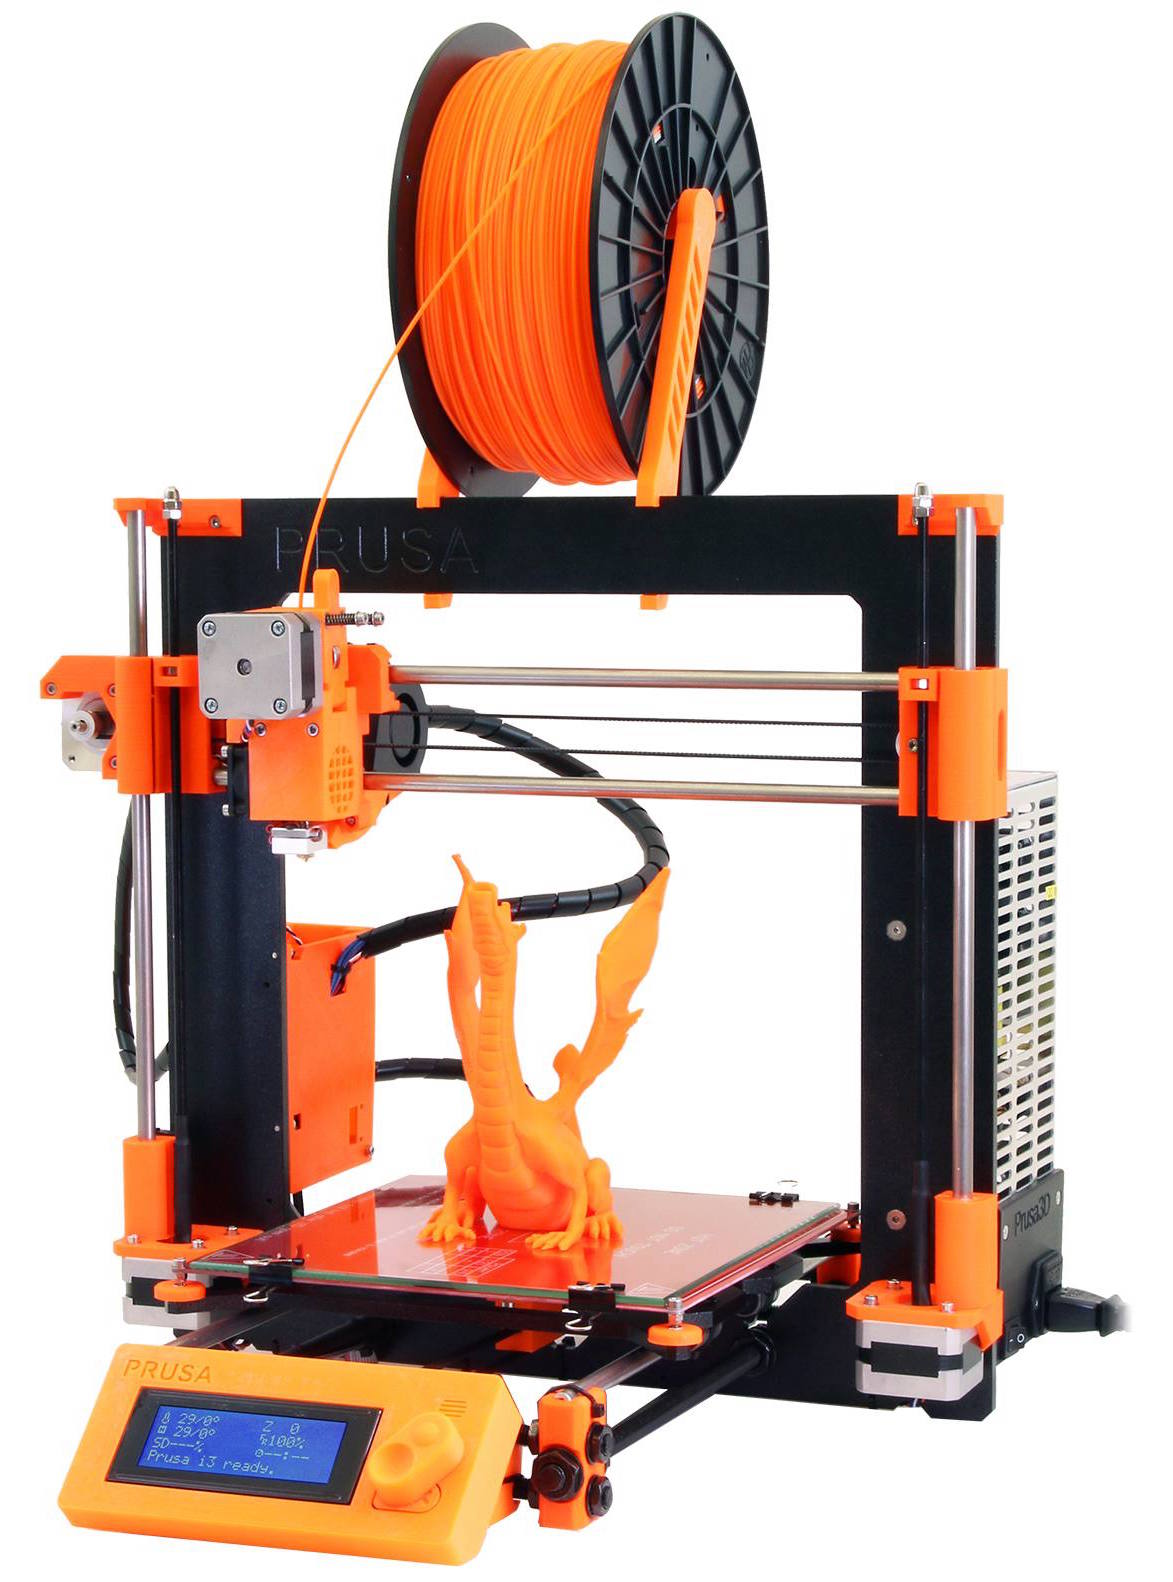
\includegraphics[width=\marginparwidth]{figures/prusai3.jpg}
  Prusa i3 - an open source 3d printer\cite{prusai3} 
} 3d printers are perhaps the most associated tools with this transformation. 3d printers, in contrast to other tools like milling machines, use additive manufacturing as opposed to subtractive manufacturing, i.e. they construct an object by adding layers of materials rather than cutting into a block of material. This allows for objects with complex inner structures to be designed and fabricated by people who are not sophisticated designers. 3d printers have gained enormous popularity thanks to their simplicity and the wide availability of cheap models. While they are far from being the ultimate digital fabrication tool, perhaps their greatest contribution is to serve a ``gateway drug'' into the world of digital fabrication. 

With widespread availability of digital fabrication tools, the world of hardware design is starting to mimic the one of software development. Online communities such as Thingiverse\cite{thingverse} and Hackaday\cite{hackaday} allow their members to share designs, learn from others, and collaborate remotely. Prototypes can be built in hours which allows for quick iterative design, similarly to software. 

The proliferation of the above tools and technologies, both in software and hardware, has given birth to a culture of makers and hackers. These individuals, coming from a wide background and carrying diverse skill sets, take pride in the ability to rapidly build prototypes in a non-commercial environment. This culture extends beyond the online communities mentioned above and into real life gatherings and spaces. 

One type of gathering strongly associated with this culture is the Hackathon. \marginpar {
  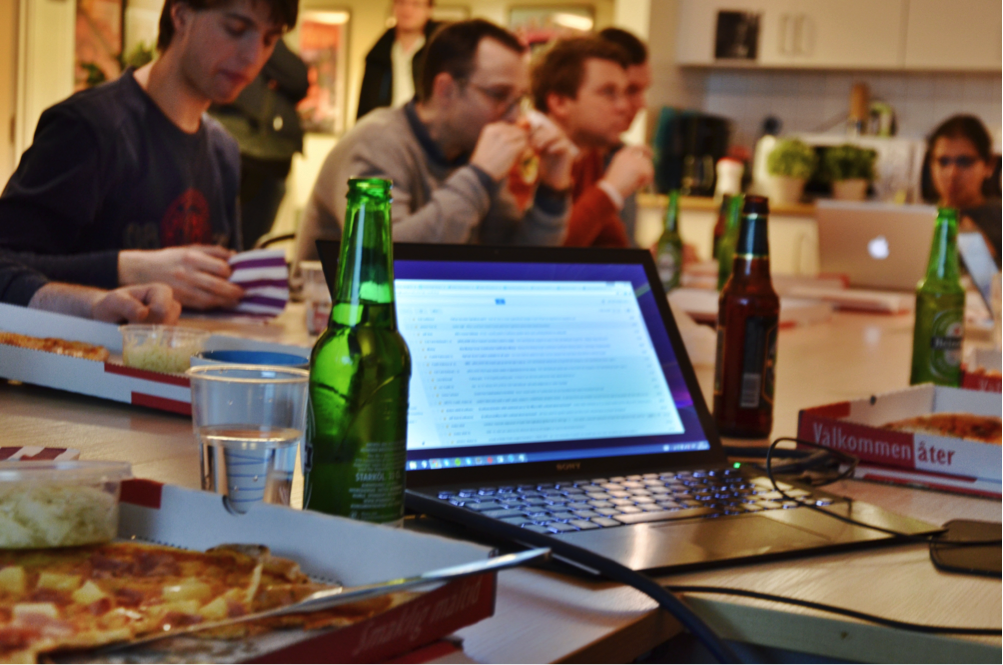
\includegraphics[width=\marginparwidth]{figures/hackathon-pizza.png}
  Hackathons often feature free pizza and beer
} Hackathons are events in which hackers gather together for a predefined amount of time, often a weekend, and build prototypes around a predefined subject. These range from commercial Hackathons, organized by companies and aimed at attracting developers to their ecosystem, to social good Hackathons, organized with a specific social goal like improving breast pumps\cite{d2016feminist} or assisting rural communities\cite{hackforwestmass}.   

The maker culture has also triggered the establishment of maker spaces. Maker spaces are physical spaces that serve specific communities by providing the infrastructure for developing software and hardware. These spaces vary in the equipment they possess, some have a single hobbyist 3d printer while others sport hundreds of thousands of dollars worth of equipment such as water-jet and laser cutters. They also vary in their economical model, some are subsidized by the host community or a corporation while other have a paid subscription model. A recent study show that there are around 1,400 maker spaces in the world as of 2016 and that number is growing rapidly\cite{makersbynumbers}.

   \begin{figure}[thpb]
      \centering
      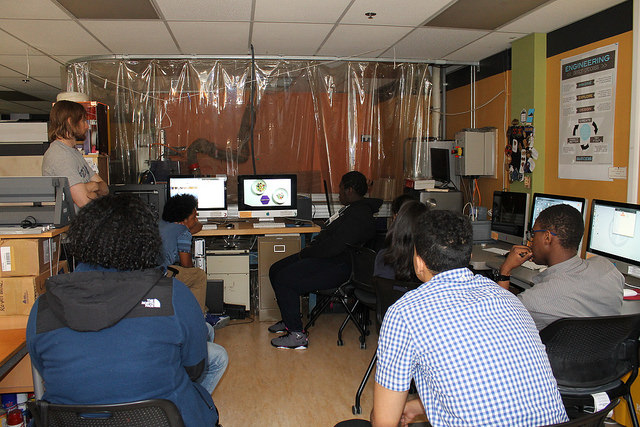
\includegraphics[width=\textwidth]{figures/setc-fablab.jpg}
      \caption{The southend technology center is a small maker space located in the basement of a residential building in Boston, MA \cite{setc}}
      \label{fig_setc_class}
   \end{figure}

   \begin{figure}[thpb]
      \centering
      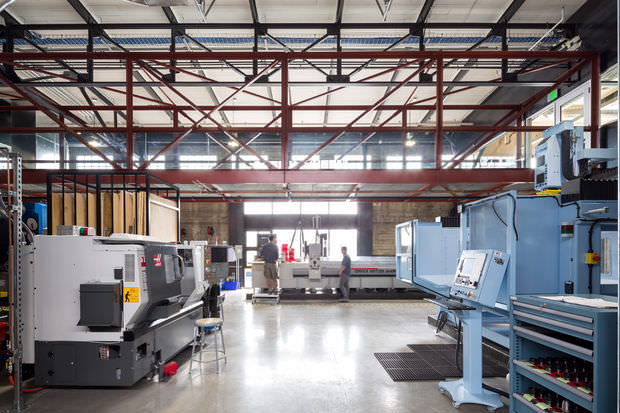
\includegraphics[width=\textwidth]{figures/pier9.jpg}
      \caption{Pier 9 is a 12,000 square-foot maker space used by Autodesk employees and affiliates.\cite{pier9}}
      \label{fig_pier9}
   \end{figure}

\section{Crowdsourcing Problem Solving}

\textit{This is How} is a crowdsourcing system for Brainstorming and Collaboration. It allows makers and nonprofits to exchange knowledge, ideas and skills, and collaborate towards problem solving. In this section I explore existing crowdsourcing systems and their various properties.

In the heart of Crowdsourcing systems are three basic constructs: Initiators, Tasks and Participants. Initiators are organizations or representatives of organizations that publish Tasks which are then performed by Participants. 

I present various examples of existing systems while characterizing these constructs. What is the motivation of initiators and who are the beneficiaries? How specific are these tasks and what level of skills do they requires? What is the nature of collaboration between participants, if any, and what is their motivation?

In this section I focus on Crowdsourcing Systems that revolve around specific tasks with a clear benefactor, similarly to \textit{This is How}, rather than general systems for collaboration management such as Wikipedia.

\subsection{Simple Tasks Crowdsourcing}

Simple Tasks Crowdsourcing systems are defined as ones where tasks are relatively simple and do not require a significant time commitment. Amazon Mechanical Turk (MTurk) \cite{mturk} is the most well known one. In MTurk, initiators, named Requesters, publish simple tasks to be performed by Participants, called Workers. Tasks carry a monetary reward and don't require any specialized skills or major time commitment. Common tasks include filling surveys and  identifying objects in pictures, these are often used in academic behavioral research.  

Not all of these systems are driven by monetary transactions. Ushahidi is a crowd mapping service driven by social activism\cite{ushahidi}. Ushahidi enables local observers to send geo-tagged reports on incidents during major events. These incidents are plotted on a map accessible via the web and essentially create heat-maps for events. These are monitored by activists and relevant authorities which can act on them. The system has been used in incidents of natural disasters as well in conflict areas during elections. 

\marginpar {
  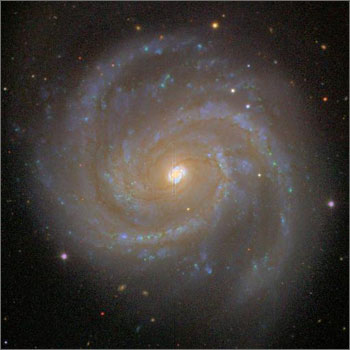
\includegraphics[width=\marginparwidth]{figures/spiral-galaxy.jpg}
  A spiral galaxy classified on Galaxy Zoo\cite{galaxyzoo} 
} These type of systems have also been used in the world of citizen science\cite{sauermann2015crowd}. Galaxy Zoo is one such system that distributes the task of classifying deep space imagery taken by telescopes\cite{galaxyzoo}. Galaxy Zoo utilizes the fact that human observation, with very little guidance, is superior to existing computer vision algorithms in classifying deep space imagery. Since it's inception in 2009, hundreds of millions of photos have been classified. 

\subsection{Bounty Based Crowdsourcing}

In contrast, In bounty based Crowdsourcing systems, tasks tend to be more complex. These systems allow Companies and Organization to publish major challenges they're faced with, along with declared bounty. Multiple participants can offer solutions but only one is chosen by the Client and receives the reward.   

InnoCentive\cite{innocentive}, one such service, is used by companies as big as Dupont and Boeing, who pay up to hundreds of thousands of dollars for creative solutions to the challenges they present. The solvers, as InnoCentive calls them, are often self taught, creative individuals who don't necessarily come from a classic research and design background. This differentiation is what drives their out-of-the-box ideas which these clients seek. \cite{howe2006rise}

Indeed, the great advantage of this approach is democratizing the space of problem solving and lowering the bias of formal training and domain expertise. Marion K Poetz et al (2012)\cite{poetz2012value} show that although crowd sourced ideas tend to be less feasible than traditional expert ones, they show greater novelty and customer benefit. 

\subsection{Distributed Design Crowdsourcing}

The previous mentioned approaches use the Internet to extend their reach, yet they do not tap it's potential of ad-hoc collaboration. Distributed Design Crowdsourcing systems allows for the formation of ad-hoc groups of collaborators working together towards a common goal.  

One of the earliest examples of such a system is ThinkCycle, founded in 2001 \cite{sawhney2002thinkcycle}. ThinkCycle was an initiative started by students at the MIT Media Lab with the aim of bringing the spirit of open source software development into the world of industrial design. It’s key component was an online shared database of problems and evolving design solutions. Similarly to challenge Based systems, each design process started from a challenge posted by a member of the community. However, rather than competing with one another, participants collaboratively came up with ideas and refined them. While ThinkCycle showed some promise it ultimately failed in sustaining a community of problem solvers.

Although ThinkCycle is not active anymore it inspired the birth of similar services. Quirky\cite{quirky} is one that is focused on home automation industry. Members can contribute to ongoing challenges and vote on the significance of contribution of other members. When a product is released all contributors share the profits according to their perceived contribution by the community. 

Openideo\cite{openideo} attempts to utilize the same methodology while tackling global issues.  Their online challenges deal with issues ranging from combating the Zika virus to improving the livelihood of small scale farmers. \marginpar {
  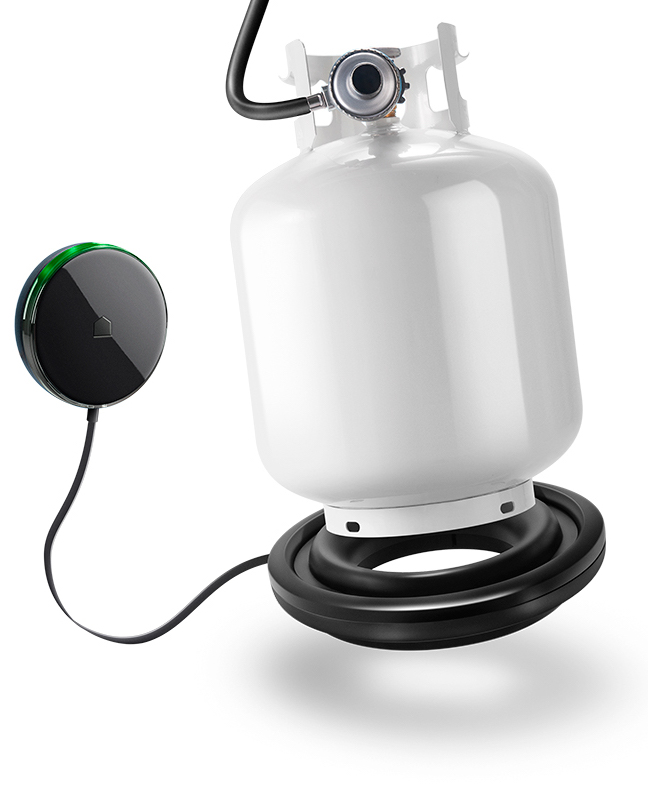
\includegraphics[width=\marginparwidth]{figures/refuel.jpg}
  Refuel - an internet connected propane tank gauge. developed on Quirky\cite{quirky} 
}

\subsection{Crowdsourcing Systems - Conclusion}

There is a variety of Crowdsourcing Systems that facilitate problem solving. These systems have various characteristics yet they share one, the specificity of the tasks they present. In all the mentioned systems, tasks and challenges are well defined. In this thesis I explore the space of crowdsourcing platforms for clients that don’t necessarily know how to articulate their problems, or indeed, that they face these problems.

\section{HyperMedia}
\begin{quotation}
``There is a joke about the man who has a map of the world ... with a scale of 1 mile to 1 mile. Sometimes video has the same character; it can be difficult to compress in useful ways. Sometimes you have to see all of it to understand any of it.''  \cite{mackay1989eva}
\end{quotation}

This is How makes extensive use of video. Video is inherently linear, it has a well defined length and pace of advancement. This creates various issues I tackle in the Design Considerations chapter. The method I will present is inspired by the world of HyperMedia. In this section I explore its history and related examples.

Since the early days of cinema, filmmakers have attempted to break down the linearity of film. Early attempts took the form of interactive cinema - A non linear cinematic experience that includes decision points in which the viewers choose one of several possible plot directions.

The first interactive cinema movie is considered to be Kinoautomat\cite{cincera1967kinoautomat}, shown in the Montreal World Expo in 1967. At nine points during the film, the screening would stop and a moderator would ask the audience to vote between two possible decisions that represent two possible scenes. The votes were counted and the winning scene would be played next.    

With the introduction of computers and digital media, such experiences became easier to implement. Moreover, they allowed the addition of hyperlinks, images and text layers in addition to the base video layer, marking the move from Interactive cinema to Hypermedia.  

The first Hypermedia experience is often credited to be the Aspen Movie Map\cite{lippman1978aspen} created at the MIT Architecture machine shop in 1978. The Aspen Movie Map was a virtual tour through the streets of Aspen, Colorado, facilitated by a touch display. A user would sit in front of the display and shown a film from the point of view of a car driving through the streets. A touch user interface allowed the user to \"turn\" the direction of the moving car, or focus on a specific building to get more data about it including text and images. 

   \begin{figure}[thpb]
      \centering
      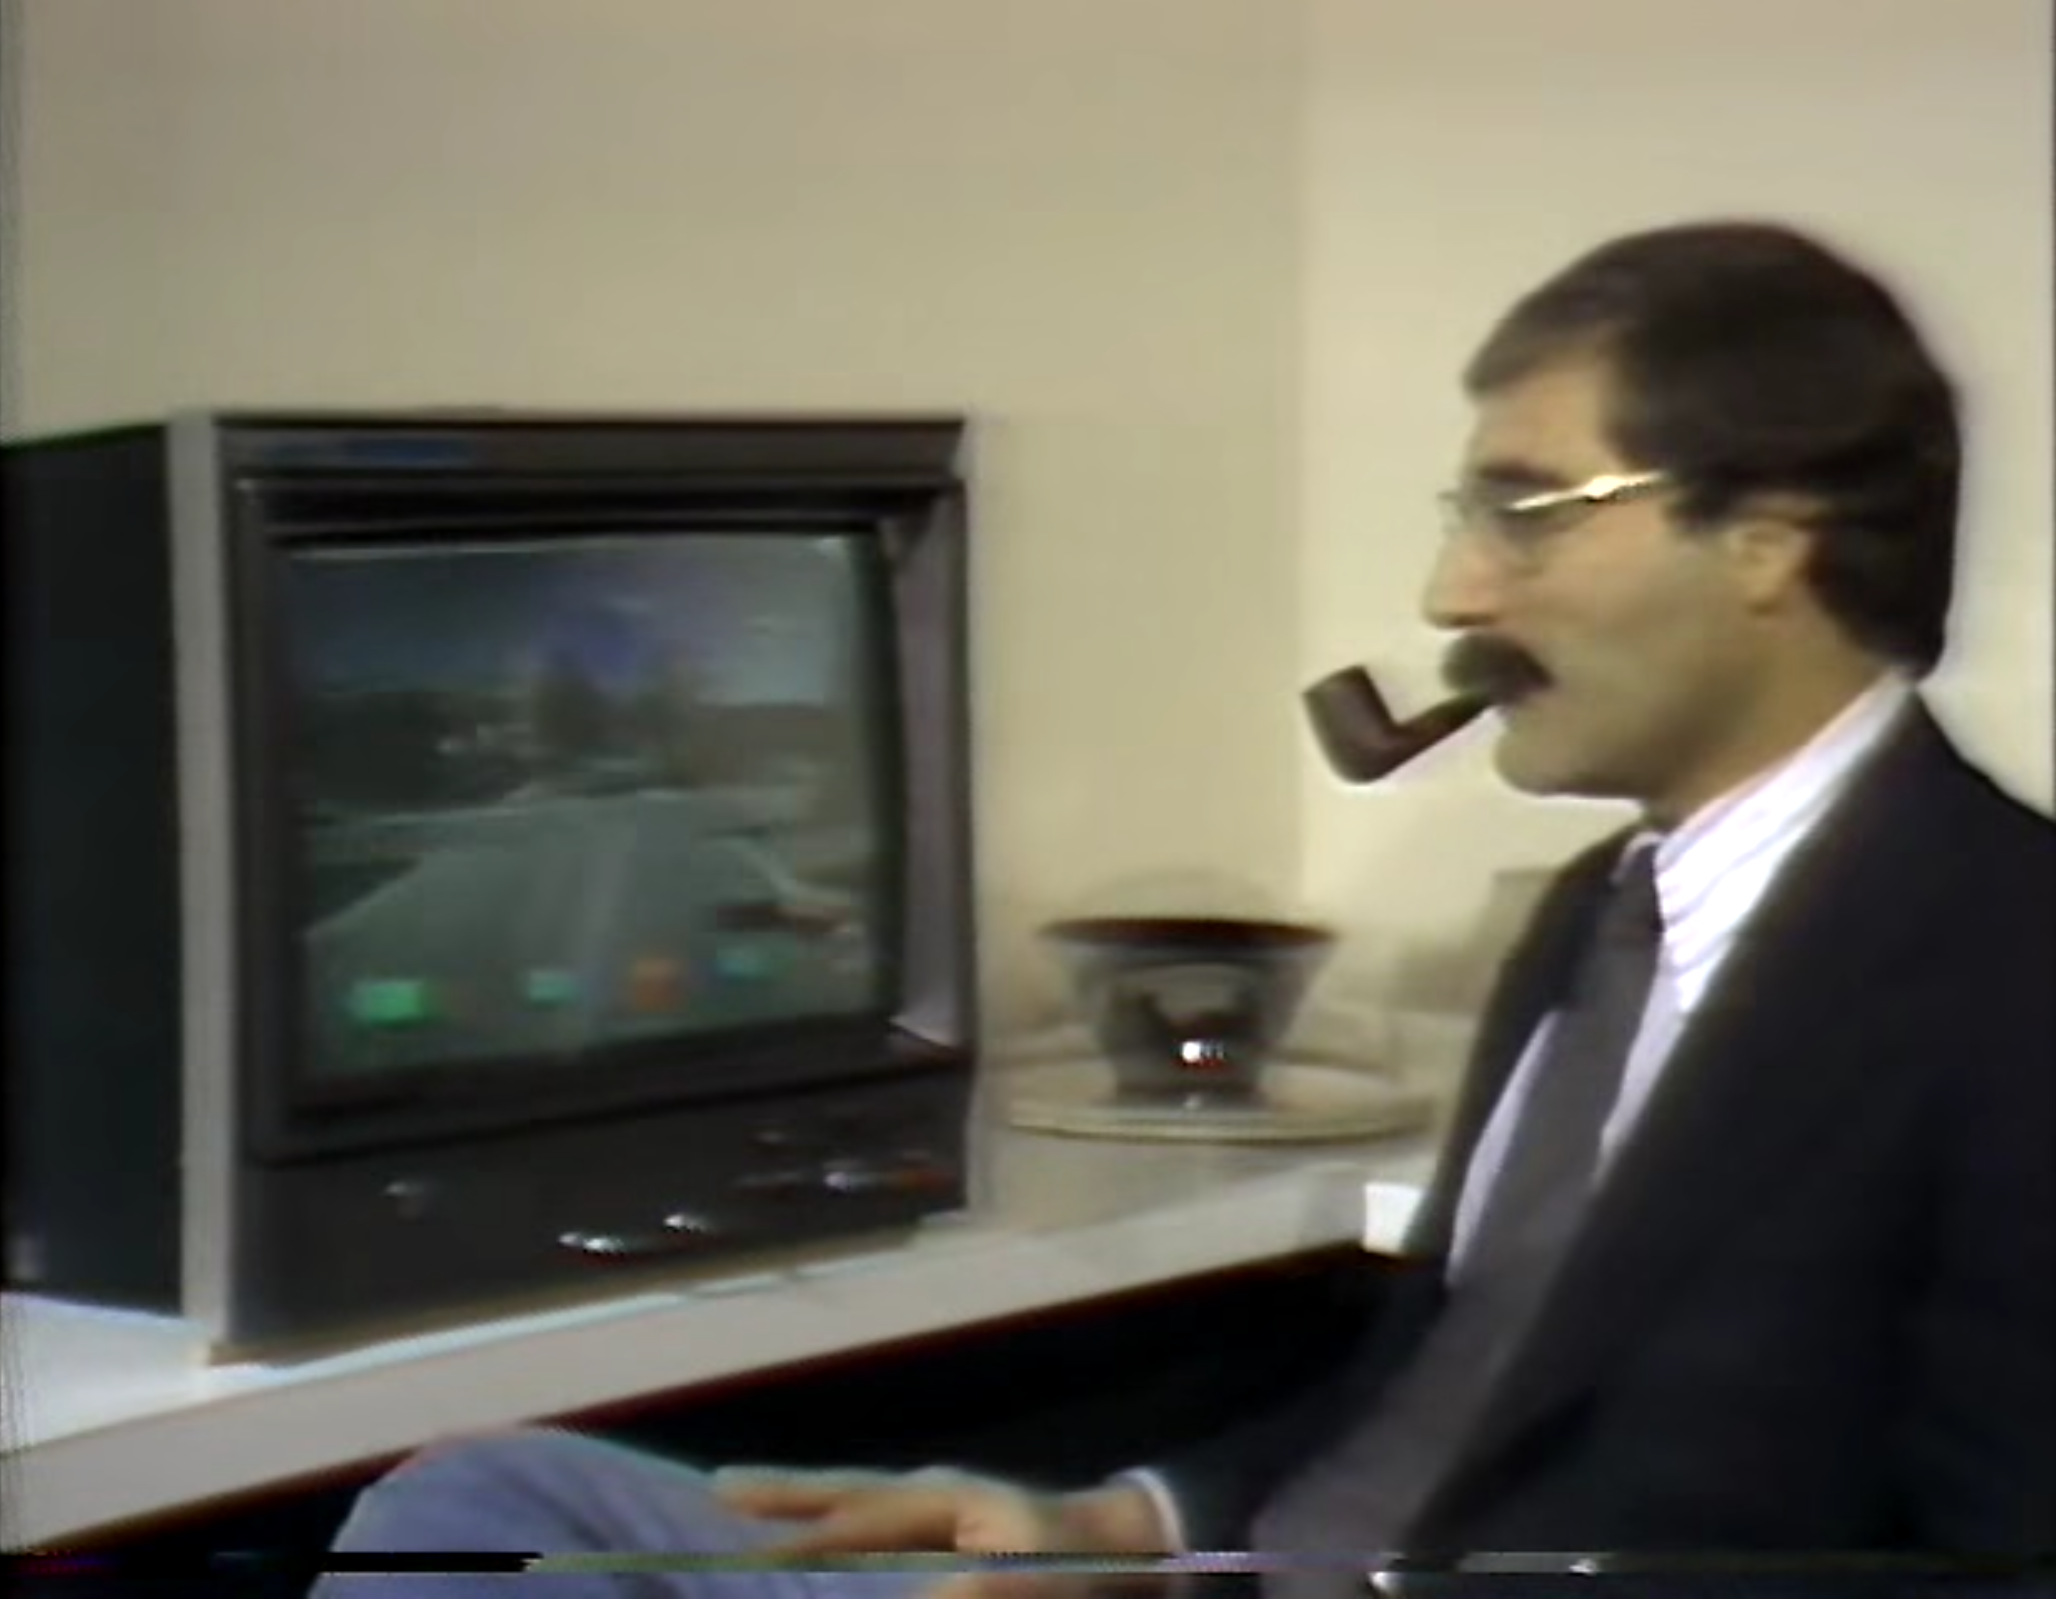
\includegraphics[width=\textwidth]{figures/aspenmoviemap.png}
      \caption{Andy Lippman demonstrating the Aspen Movie Map (1981)\cite{lippman1978aspen}}
      \label{fig_pier9}
   \end{figure}

Hypermedia stayed a focus of the Architecture machine group as they transitioned and became the MIT Media Lab. One notable project led by Glorianna Davenport, was \textit{The Elastic Charles}\cite{brondmo1990creating}, a HyperMedia experience that revolved around a time-lapse journey down the Charles river in Boston. Fifteen students contributed to the project by placing hyperlinks to text, graphics and extra video content on a base film, corresponding to the location portrayed in it. 

With the introduction of the Web, the distribution of HyperMedia using standard technologies became easier. The popular video distribution platform Youtube\cite{youtube} allows video creators to place simple hyperlinks on a specific time and location in their videos that link to other videos published by them. Platforms such as Interlude\cite{interlude} take it a step further by making it easy to create and publish nonlinear videos, where users can make plot decisions and control which scenes are displayed next. Popular streaming service Amazon Video \cite{amazonvideo} have began overlaying TV Shows with hyper links to learn more about the actors relevant to specific scenes being watched.

The above examples show a mixture of two types of interactivity in HyperMedia. In one, such as in Kinoautomat or Interlude, the base video layer can be manipulated by user interactions. In the second, such as in The Elastic Charles, the base layer is static but is overlaid with additional layers of media that provide further information and interactivity. The Aspen movie map combines both. In this thesis I focus on the latter.  




\chapter{Outlining Story centric Brainstorming and Collaboration }
\label{chap_anatomy}

This thesis proposes a system for story-centric distributed brainstorming and collaboration. Story-centric collaborations between makers and nonprofits are collaborations that are a result of the stories told by nonprofits. These stories represent the goals, processes and constraints of the nonprofits. While these nonprofits will not always have the expertise to define a challenge a specification of a solution, they are well versed in articulating their story.

Before designing a distributed system it is crucial to understand how these type of collaborations work in small scale. To that purpose I present three case studies of story-centric brainstorming and collaboration. These case studies are based on testimonials from relevant organizations and participants through unstructured interviews. At the end of the Chapter I present my impressions and a common process extracted from these cases. 

\section{Milky}
This case study represents my own experience in working with the Mothers' Milk Bank Northeast \cite{mmne}. This collaboration started in the summer of 2015, before my thesis research started, and served as motivation for the research direction I chose.

The Mothers' Milk Bank Northeast is a non profit community organization that receives donations of human milk, processes them and provides them to babies in fragile health throughout the Northeastern United States. Breast milk is considered to be the healthiest source of nutrients for babies and especially important in cases of preterm birth, infectious disease and various other medical conditions.\cite{lewandowski} However, for various reasons, sometimes the birth mother can not lactate. The milk bank collects donated milk and makes it available through hospitals. 

I learned about the milk bank completely by chance. My peer, Tal Achituv, had co-organized a hackathon which was dedicated to the improvement of breast milk pumps \cite{d2016feminist}. One of the attendees, Yavni Bar-Yam, was the son of Naomi Bar-Yam, who runs the milk bank. Yavni told Tal about the organization, who in turn convinced me to come for a visit. I had just finished my first year as a grad student at the media lab and had an itch for industrial design and hardware fabrication.

In the visit, we learned about the process breast milk donations go through from collection until being received in hospitals. This included processing of the milk: mixing it, pasteurizing and bottling. One of the things we noticed was that the tools used by the lab workers were very basic. The milk was hand poured through a series of vessels and finally into the bottles, where the main measurement tool was eyeballing the volume markings. 

   \begin{figure}[thpb]
      \centering
      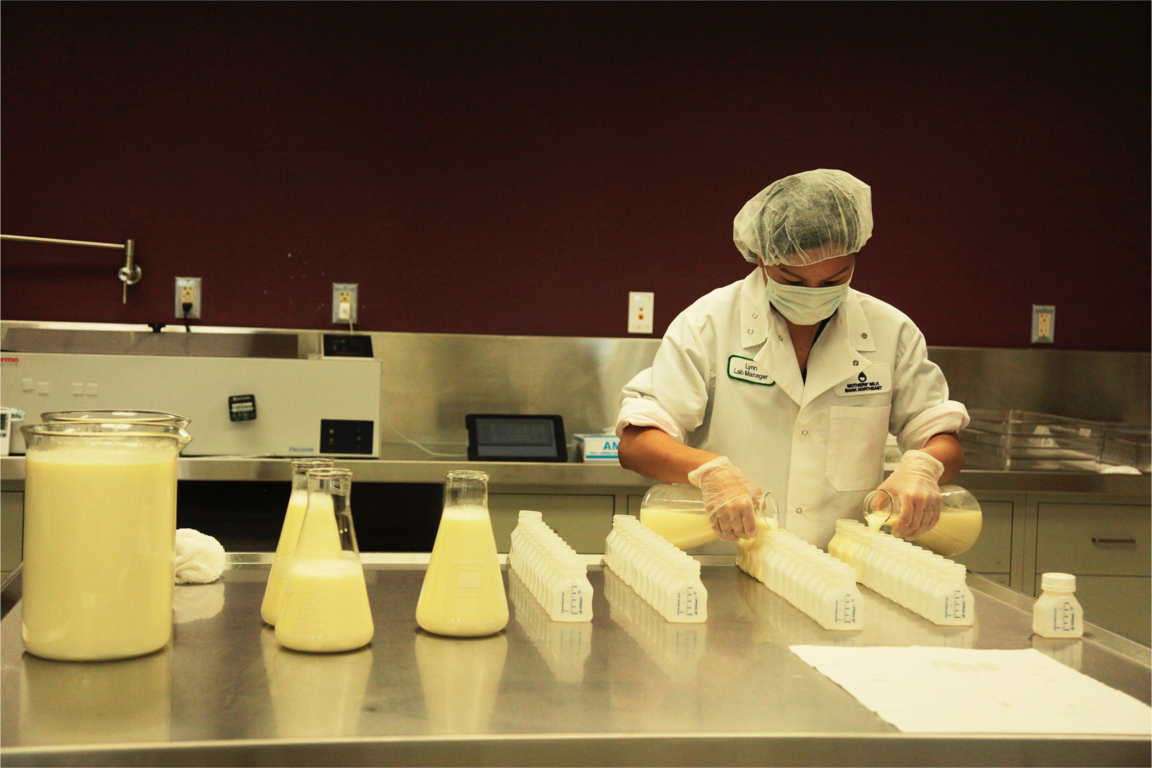
\includegraphics[width=\textwidth]{figures/mmne-manual.png}
      \caption{Manual pouring of milk in Mothers' Milk Bank Northeast}
      \label{mmne-manual}
   \end{figure}

This manual process became the focal point of our discussion. While it was cumbersome it also presented issues of accuracy and being prone to infections. The milk bank had tried to address these issues before using an off the shelf peristaltic pump instead of manually pouring. However, it slowed down the pace of work and did not allow for parallelization between lab workers. 

We suggested a simple solution for the problem, building a carousel bottle feeder in conjunction with a peristaltic pump. The carousel will allow continuous feeding of empty bottles on one side and capping and removing the bottles on the other side. We called this device Milky. 

   \begin{figure}[thpb]
      \centering
      \includegraphics[width=\textwidth]{figures/milky.png}
      \caption{Milky - Early Prototype}
      \label{milky}
   \end{figure}

We built several iterations of Milky during a period of several months while being in constant dialog with Milk Bank. We did so in collaboration with the organization's employees. The lab workers, who will eventually use the machine, gave us feedback early along the process to make sure the device fits in the lab and is suitable for their work flow. Professor David Newburg, who is the research advisory board member for MMNE advised us regarding the materials we used, sanitation issues and made sure that the process does not prove to be harmful for the milk. 

Milky itself hasn't been deployed due to the delicate nature of the operation and a necessity for continuous on site support requirements. However, the continued process of brainstorming and collaboration has led the milk bank to commission an industrial quality version of it from a local engineering firm. The specification for this machine were outlined in collaboration with us, based on the insights from our continuous brainstorming and experimentation process. This machine is scheduled for deployment during September 2016.

For me, this was an invaluable experience. I got a chance to utilize my newly acquired skills and have a real world impact.  In developing Milky, I became convinced that there is an unrealized opportunity for makers and nonprofits to collaborate in a way that could be beneficial for both parties.

\section{Laser Painting}

Deborah Dawson, an artist from New York, helps kids with cerebral palsy to create art. She does so by attaching a small laser pointer to their heads and have them point at a painting canvas. In turn, she traces their pointer to create an abstract painting. This allows kids with very little ability to express themselves, to create art they can call their own.

   \begin{figure}[thpb]
      \centering
      \includegraphics[width=\textwidth]{figures/laser-session.png}
      \caption{Deborah Dawson in a Laser Painting session}
      \label{laser-session}
   \end{figure}

However, Deb  has had a continuous challenge with mounting these devices. Laser pointers are not designed to be worn on the head. This proves to be very difficult, especially by kids that suffer from cerebral palsy and have limited motor skills. Her quest to find a more suitable alternative led her to companies that manufacture lasers sights built for guns. Naturally, these companies could not help. Eventually, on a long shot, she sent an email describing her issues to an MIT Media Lab Prof., Ros Picard, who in turn sent it to all Media Lab students. 

Tal Achituv, spotted that email and invited Deb to MIT. Deb, Tal and several other students, including myself, met with her. We learned about her work and suggested a headband design with an integrated low power laser pointer for the kids. Moreover, through our conversation we learned about her entire operation which led to a discussion over some other challenges she faces. For example, the fact the she worked in different schools and in different spaces meant that all the equipment needed to be carried around. Not to mention, locating spaces that had the accessibility requirements for these kids was also challenging. One of the ideas we discussed was repurposing an old school bus with wheelchair accessibility and the painting infrastructure. That way the equipment only needs to be setup once and the bus could travel around New York and cater to various schools in different locations. 

   \begin{figure}[thpb]
      \centering
      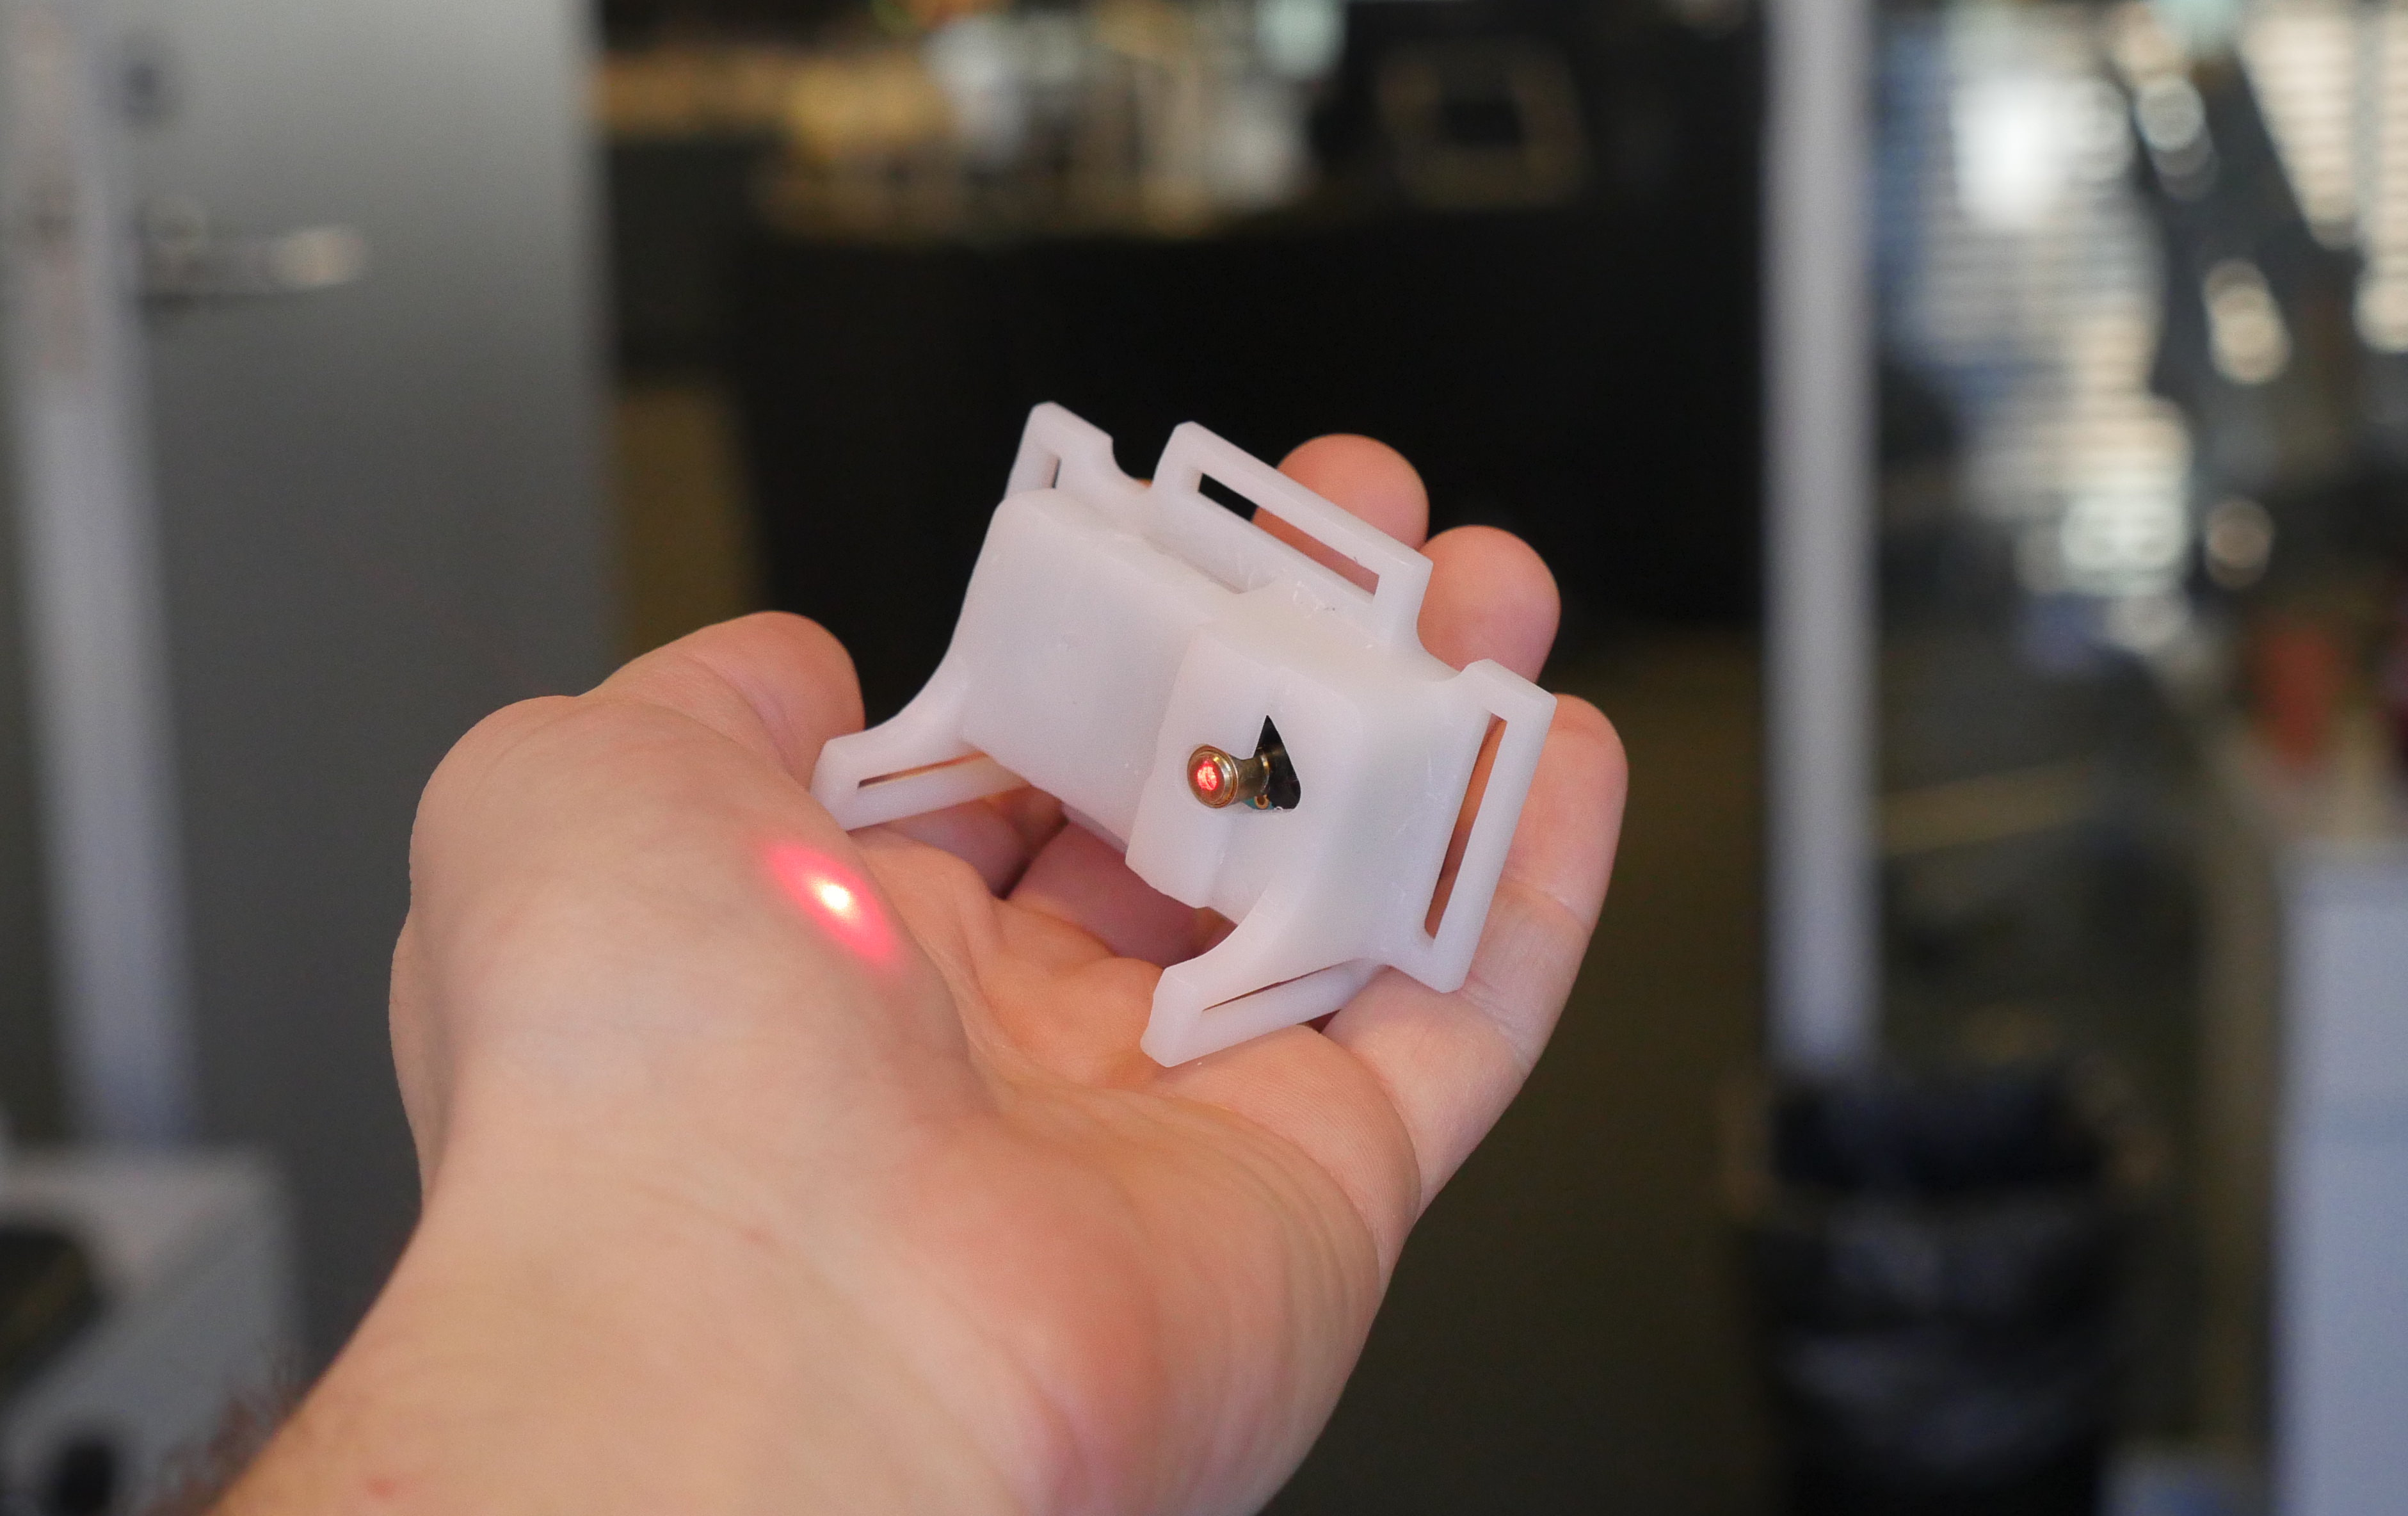
\includegraphics[width=\textwidth]{figures/new-laser.jpg}
      \caption{Improved Laser apparatus for Laser Painting. Includes a remote kill switch and  various mounting options.}
      \label{new-laser}
   \end{figure}


The alternative headband laser pointer was delivered to Deb in the Spring of 2016 and has been in use since then. Moreover, Deb is currently looking to expand her operations and is in touch with maker spaces in New York to fabricate more of them. Also, Deb is actively seeking funding for the re-purposing of a bus as a portable studio for her work. 

This collaboration has also inspired Tal to further explore the world of assisted self expression.  For his thesis project he built a painting machine that assists people with various disabilities to express themselves by drawing, with minimal assistance from other people\cite{projexpress}. 

   \begin{figure}[thpb]
      \centering
      \includegraphics[width=\textwidth]{figures/express.png}
      \caption{Project \textit{Express} - Self assisted painting machine}
      \label{express}
   \end{figure}

From this collaboration I learned that while nonprofits will often seek help with a small, narrow challenge, there is an opportunity for both parties in discussing the bigger picture: the story. 

\section{Cradles to Crayons}

Following the previous two study cases, I set out to initiate a more structured exploration into the space. In contrast to our previous experiences, which happened somewhat serendipitously, this time I actively sought out a potential collaboration. 

The initial challenge was to find a suitable organization. Given that nonprofit organizations matched the profile, I approached the Massachusetts Nonprofit Network (MNN). The MNN agreed to publish a call for collaboration in their weekly newsletter which yielded some 50 requests from various nonprofits. In the requests, one stood out as having a complex ground operation that might be of interest to makers, Cradles to Crayons.   

Cradles to Crayons (C2C) provides children from birth to age 12, living in low-income and homeless situations, with the essential items they need to thrive – at home, at school and at play. They supply these items free of charge by engaging and connecting communities that have with communities that need.

The C2C operation is logistically complex. It starts with donation bins distributed in local communities and goes through sorting and filtering in their main facility, and ends in creating custom packs for children in need, which are distributed through local social workers. 

I arranged for a party of 15 makers to visit the C2C facility in Brighton, MA. These were reached through my personal network at the Media Lab and maker-spaces in Boston, they expressed interest in learning about nonprofits and their skills varied from Software Engineering to Mechanical Engineering and Art. The tour was led by Julia Boyaval, director of community engagement for C2C, who received no instructions apart from showing us around the facility the same way she would in any other circumstance. During the tour the participants learned about the different challenges the organization faces: from the security of their donations bins to difficulties of managing stock. This learning process was backed by a continuous discussion between the participants, Julia and other employees of the organization. 

   \begin{figure}[thpb]
      \centering
      \includegraphics[width=\textwidth]{figures/c2c-tour.jpg}
      \caption{A Maker tour of Cradles to Crayons}
      \label{fig_setc_class}
   \end{figure}

At the end of the tour the participants gathered in an office to discuss. Given that C2C have a complex operation, the first thing they did is formalize the entire operation as a block diagram on a whiteboard, utilizing one of the participants as a moderator. Next, each participant was given a sticky note to write one idea on, and stick it on the whiteboard around the most relevant block. This quickly formed clusters of sticky notes around identified blocks and triggered a discussion about the different problems and the various proposed solution. 

   \begin{figure}[thpb]
      \centering
      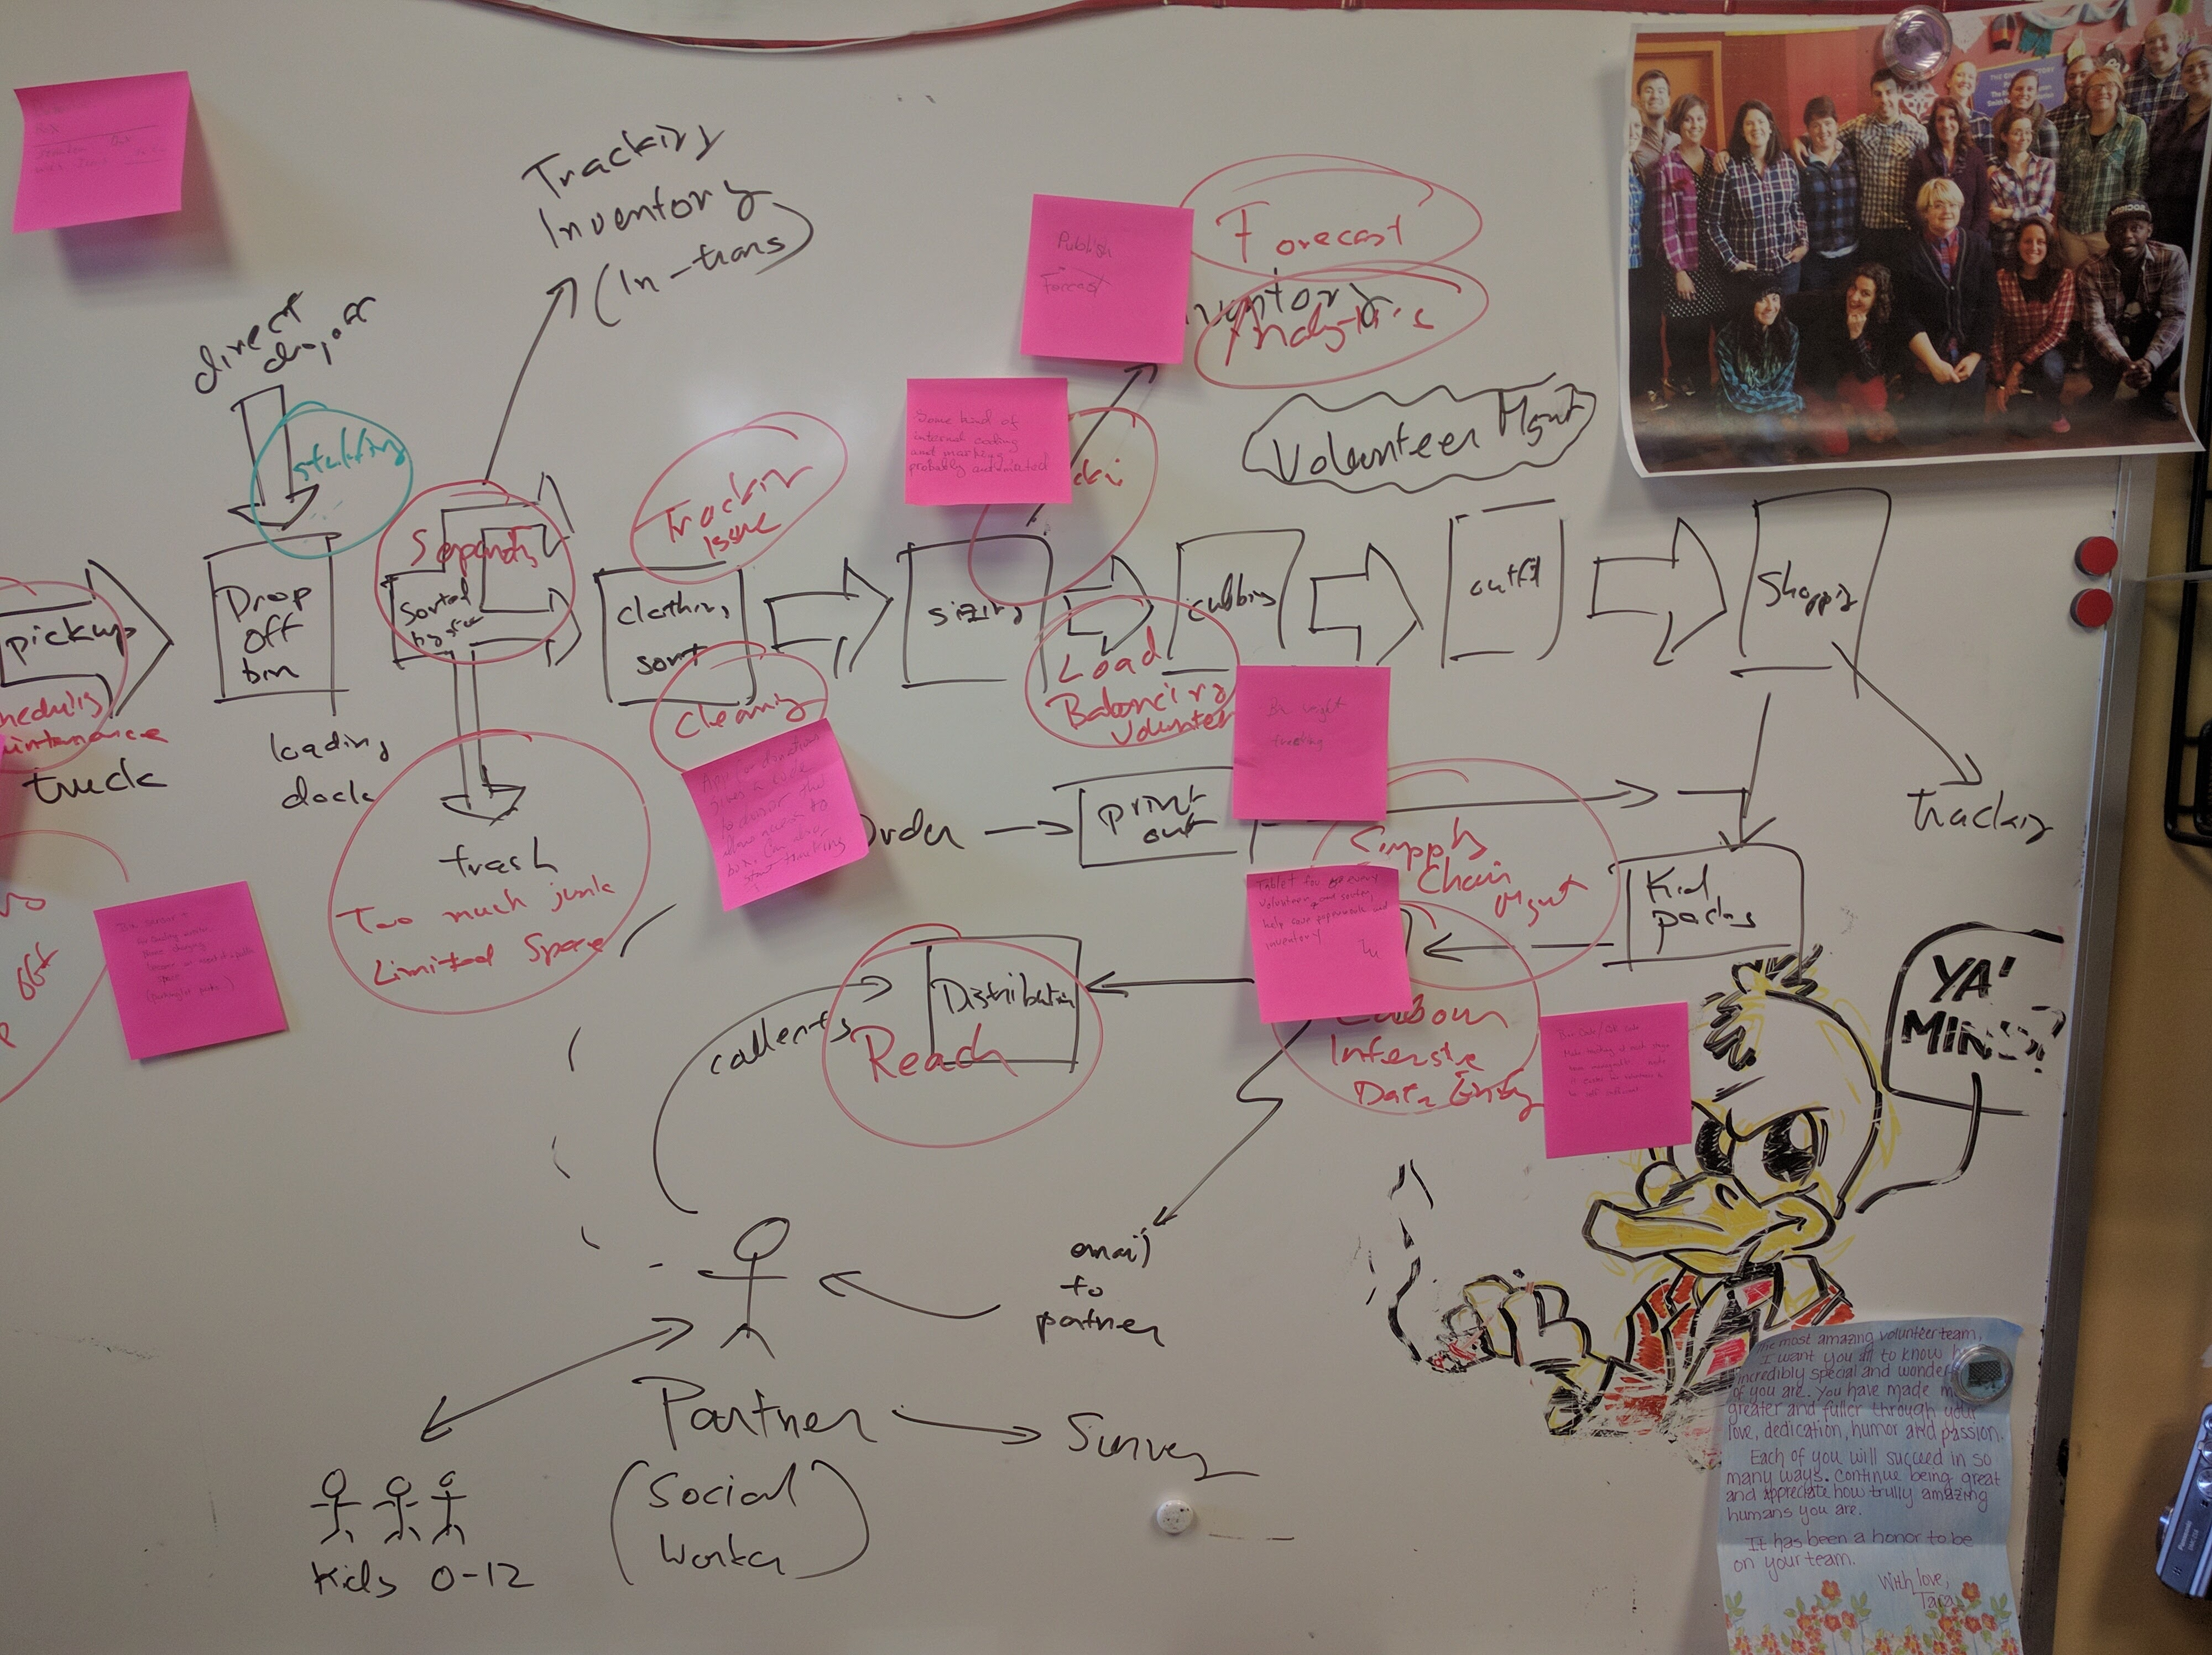
\includegraphics[width=\textwidth]{figures/c2c-brainstorming.jpg}
      \caption{Whiteboard post Cradles to Crayons brainstorming session}
      \label{fig_setc_class}
   \end{figure}


The proposed ideas varied in nature. One of them, a mobile application, tackled the inventory issues by allowing donors to create a manifest of their donations in advance. Another, suggested creating a direct link, using a mobile app, between the donors and the social workers, thus reducing congestion in the facility. Others were as simple as modifying the graphics on the bins to better instruct the donors what belongs in them and what doesn't. 

At the end of the tour several of the participants expressed interest in working with C2C although none of them are currently engaged in such collaboration, citing time constraints as the main barrier. With that said, the event was still successful as the idea of creating a direct link between donors and social workers through a mobile app has been approved by management and is in an initial phase of implementation by the organization. The congestion challenge this app addresses was not part of the challenges originally laid out by Julia but rather surfaced from the broad story of the organization, showing the power of these stories.  

This exploratory collaboration has taught me about the different nature of nonprofits. While the previous two case studies addressed small nonprofits, C2C is a different story. They are a national nonprofit with close to a hundred employees, three large scale distribution centers and tens of thousands of donation packages processed per week. At such a scale, experimenting is non-trivial and failed experiments might might negatively affect the organization’s core services. 

\section{Impressions}

Examining the above cases demonstrate that the concept of story-centric brainstorming and collaboration works towards the goals I stated in the introduction chapter. All the nonprofits mentioned have stated that they have gained a valuable different perspective on the challenges they're facing while learning about the abilities and skill sets of the makers they've worked with. In turn, the makers learned about the different operations of these nonprofits and how their skill sets can help improve them. Even in cases where the collaboration itself has not produced a successful artifact, they still had an significant impact on all parties involved. 

\section{Formalizing the process}

Based on these three case studies I present a common process that has three phases. While these cases focus on nonprofit organizations on the one side, and participants with engineering backgrounds on the other side, there is still some variance in the different challenges and nature of collaboration. I believe this process is generalized enough to be used to tackle various challenges with different organizations and participants. 

\begin{enumerate}

\item \textit{Discovery} - Discovery is perhaps the most elusive step of this process but is a basic requirement for its existence. In the two first cases discovery happened somewhat by chance while the third one was the result of an intended search. How do organizations learn about the existence of these type of participants and vice versa? Moreover, how do you encourage them to engage with one another? 

\item \textit{Exploration} - In all of the above cases, participants had at least one on-site visit with the respective organizations. These explorations started from a general overview and ended in a detailed drill down into the processes employed by the organization. Open discussion during this exploration plays a major role in understanding the organization: motivation, processes and constraints. 

\item \textit{Collaborative Brainstorming} - The next step in all of these examples is a process of collaborative brainstorming. This included tossing around many ideas and, filtering and refining them according to the given constraints. Brainstorming sometimes began in a spontaneous meeting right after the exploration phase but also went on to remote forms of communications be it phone, email etc.

\item \textit{Co-design} - This final step represents an ongoing relationship of design and refinement in which a prototype is built by makers, evaluated with the nonprofit and so forth. This process is present in the first two case studies examined yet is absent from the third. While initially it may seem like the most important step, the case studies show that that there is still significant value in the process without it. 

\end{enumerate}
 
Having established that these type of collaborations work towards the goals I stated, the next challenge is to translate the outlined process into an online experience that can be scaled while preserving the unique properties of the real life experience. From here on, I will focus on the first three steps of the outlines process given that they provide a basis for collaboration and have shown to provide value on their own.
\chapter{Design Considerations}
\label{chap_design_consider}

In this Chapter I argue that video is the ideal storytelling medium for \textit{This Is How}. I will also iterate over the three steps of the process that were outlined in the the previous chapter and present design considerations for each with regards to video as a medium. 

\section{Choosing a medium}

This is How is a story centric crowdsourcing platform. Given the centrality of storytelling to the process, it’s critical to ask what medium is best for conveying these stories?

The stories presented by nonprofits in the previous chapter were told in person and in an informal manner. No structure was forced yet it did exist. It was imposed by the experience of the nonprofit in presenting their work,  a grasp of their goals and familiarity with processes. For makers, the ability to intervene and ask questions, explore and touch the surrounding, was keen for a deep understanding of the organization, their challenges and constraints. 

This full sensory experience is difficult to translate into the virtual realm with today's technology. How can we create an experience that is as expressive, natural to the stakeholders, provides an understanding of the surroundings and allows for contextual discussion?

\section{Video}

Video is expressive and raw. To understand a story, it is crucial for participants to have an unfiltered point of view. Often times the observations participants make relate to items they have seen in the surrounding and not to the main narrative the organization is trying to tell. While text often has a clearer message to it, it has already been digested to fit the narrative of the author. While the same can be said about edited video content, there is still an inherent feel of the surrounding to the medium. <TODO: find a  reference to support this statement>

%TODO: use this {https://www.psychologytoday.com/blog/behind-online-behavior/201505/video-vs-text-the-brain-perspective}

Beyond that, it is important to use a medium that users are already familiar with. Online video is extremely popular and familiar. Every minute, 500 hours worth of video are being uploaded to Youtube\cite{youtubestats}, the most popular video sharing online service. It is clear that people are capturing video. Nonprofits also already have the basic tools needed to participate: a recording device in the form of a smart-phone and in many cases broadband Internet access. 

\subsection{Limitations of Video} 

Video is far from being a perfect medium. While many nonprofit organizations might demonstrate a high level of present-ability, there is no guarantee that their ability to produce these videos will match. Creating compelling video content is difficult. A good video should strike a balance between duration and depth that makes is easy to digest yet presents enough details to get participants interested. 

The above issue is worsened by the linear nature of video, the fact that it has predetermined duration and pace makes is hard to skim over and explore. This also raises concern regarding the ability to create contextual discussion. How can we facilitate discussion over specific objects in space and time?

I'll revisit some of these issues and suggest ways to address them in the following sections.

\section{This is How}

As part of this thesis I built a web platform, \textit{This is How}, that allows nonprofits to upload a story in the form a video. This story describes the work of the organization and the processes they employ. It will also allow makers to browse through these stories, engage in discussion with the organization to deepen their understanding, and finally, collaboratively brainstorm. 

In the next three subsections I drill down into the design considerations of each of the steps we outlined in Chapter 3: Discovery, Interactive Exploration and Brainstorming. These consideration include requirements, related work and my approach. 

\subsection{Discovery - Video Metadata}
In all of the cases examined in the preliminary study, discovery is one of the most challenging issues. This is How uses metadata as a driver for discovery. 

<TODO: add some more citations about metadata>

Video contains an abundance of informations: topics discussed, number of people in it, subtitles, scenery, sound track and the exact timestamps of all of the above. This data is commonly referred to as metadata. Tapping into this data and indexing it allows for searchability and semantic linking. If the topic discussed in a story is bottling milk, perhaps a juice startup can also benefit from the knowledge?

However, detailed metadata is usually not present in videos, especially not in amateur ones. In addition, it is cumbersome to manually add metadata and one cannot expect users to manually input all this information.

The solution I propose is to employ an automatic metadata generator that will work in conjunction with simple manual data input, to generate a list of tags per video. These tags will be generated according to identified entities, both through extraction of keywords from transcribed text and through image recognition techniques. The tags, for example such as \textit{Bottle} or \textit{Donation}, can be used to browse stories by a tag filter. In the future, tags can also be used create semantic links between different stories.

\subsection{Interactive Exploration - HyperMedia}

In the interactive exploration part of the process I wish to address two of the main issues related to the chosen medium of video. How to enable contextual discussion and allow for easy exploration? Following is a review of related work and a proposed approach. 

Regarding contextual discussion, Some video viewing platforms, such as Youtube, address the contextual discussion issue using hyperlinked timestamps. This means that in the regular, linear, commenting systems, users can mention timestamps. These timestamps, for example  \textit{1:20}, will automatically be hyperlink to the relevant time in the video. In the case of \textit{1:20}, clicking on it will seek the video to one minute and twenty seconds. 

   \begin{figure}[thpb]
      \centering
      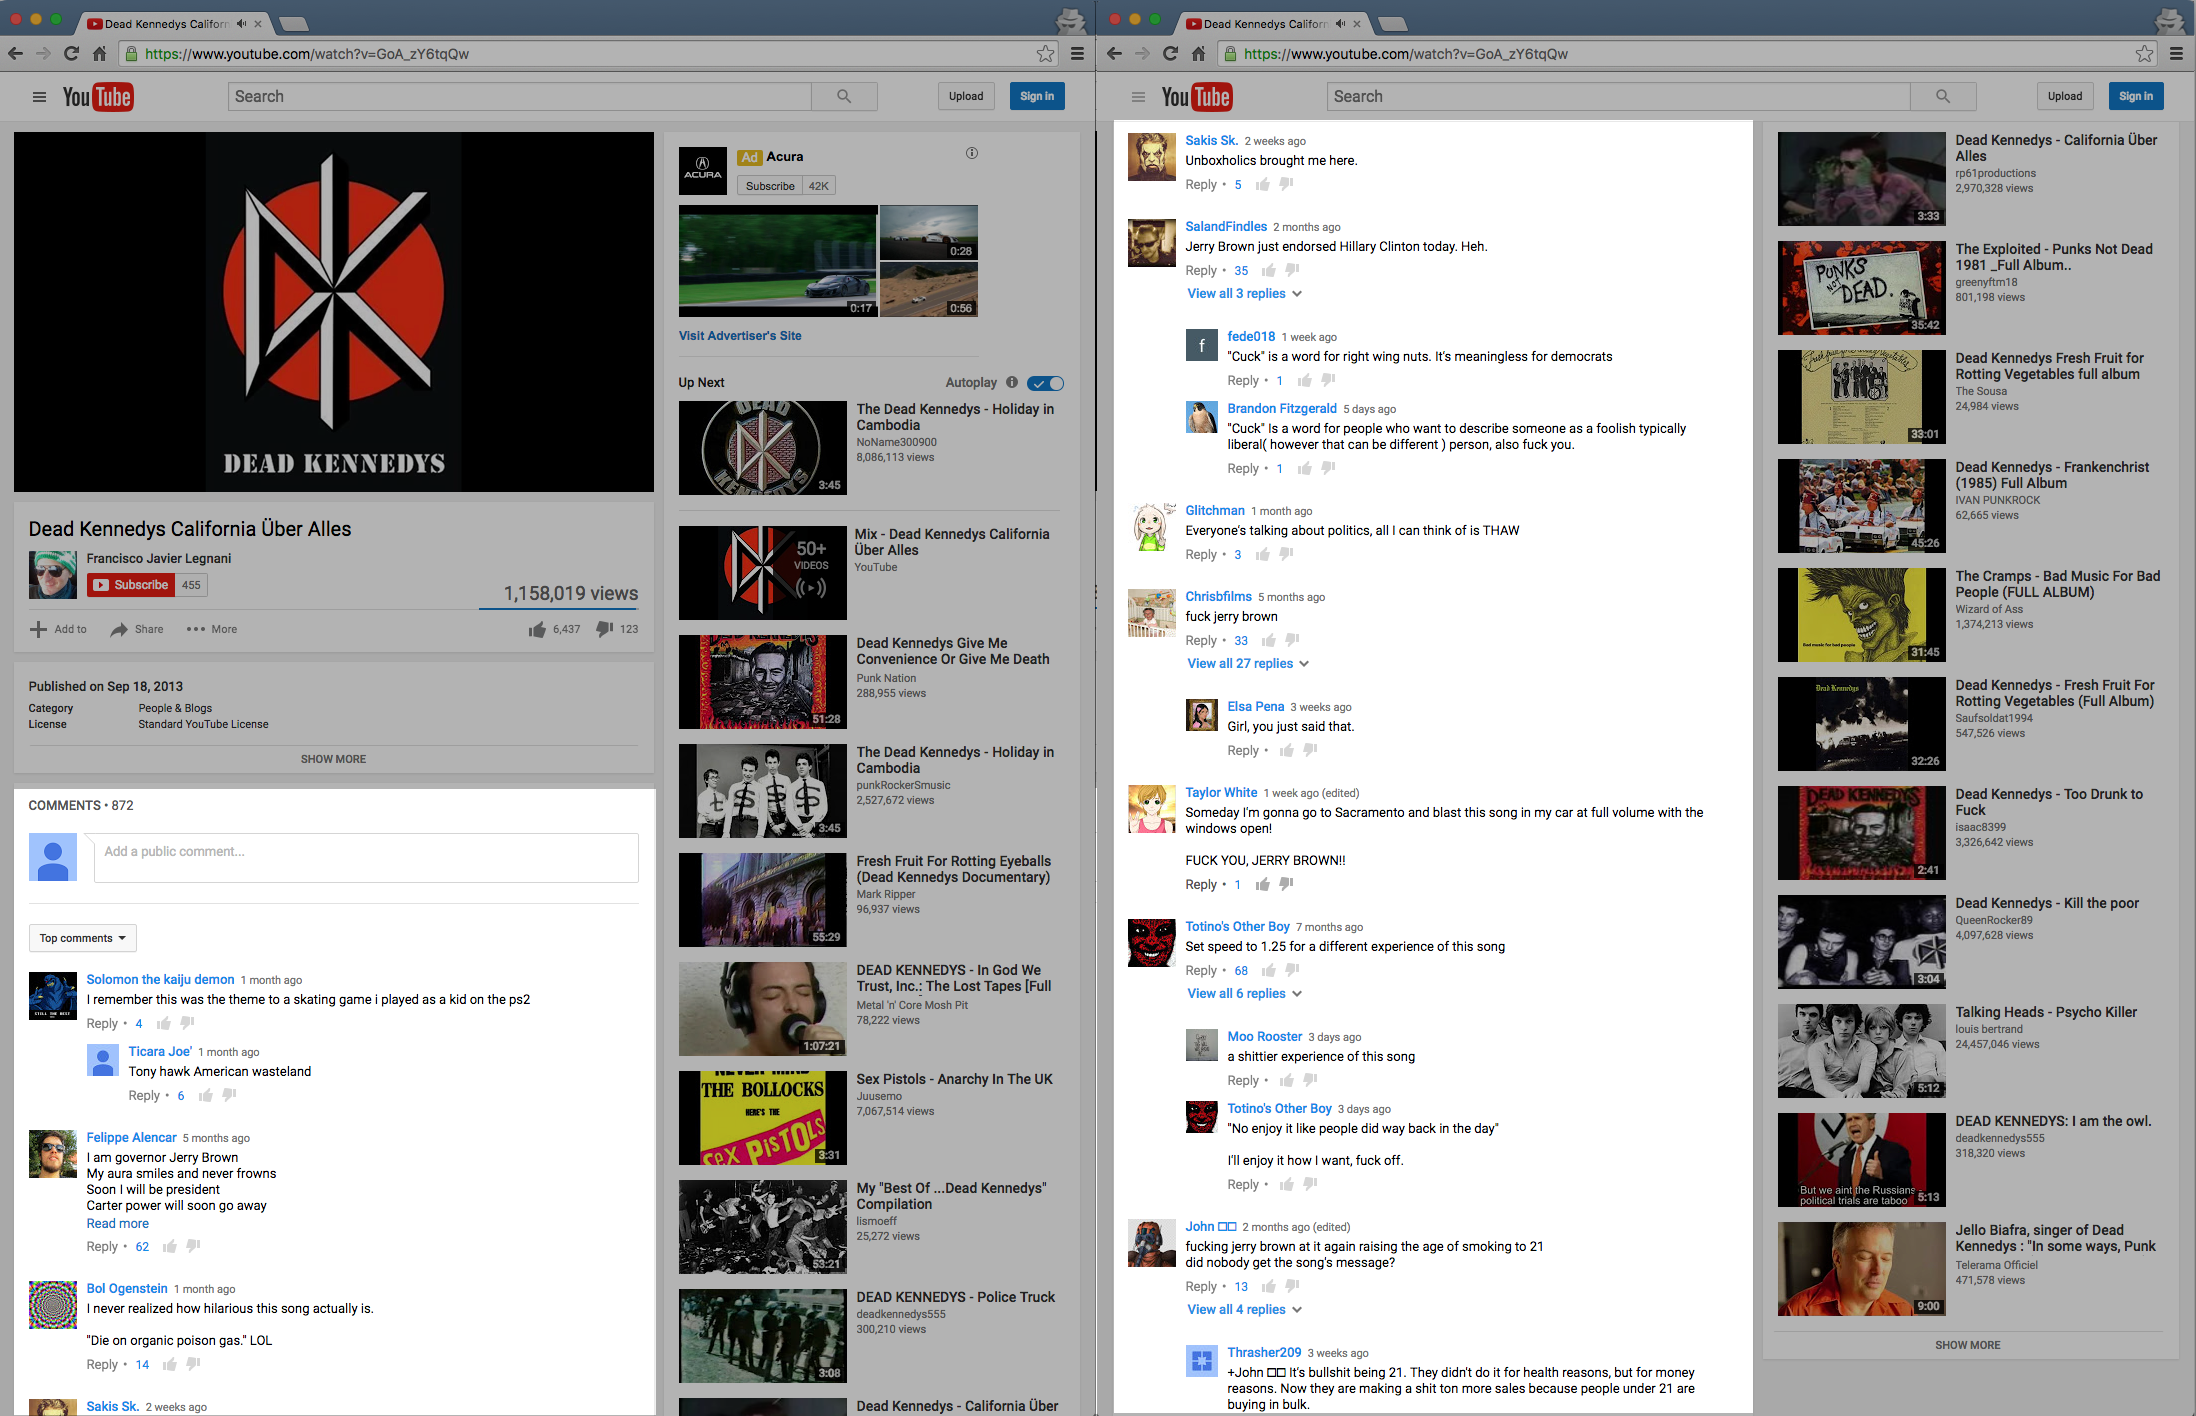
\includegraphics[width=4in]{figures/youtube-left.png}
      \caption{Youtube comments. First page is on the left, second is on the right}
      \label{fig_youtube_comments}
   \end{figure}

While this does allow for the addition of time context, these comments behave just like any other. They are presented in the order in which they were inputted, there is no indicator about their existence at playtime or when clusters of them appear and they are generally second class citizens in the video playback experience

Soundcloud \cite{soundcloud}, a music streaming service, attempts to solve this issue. They place indicators of timestamped contents on the seek bar of the audio clip. The actual comment text is displayed when the playback timestamp matches that of the comment or when the listener hovers their mouse above the indicator. This approach puts comments in the front of the experience and results in clusters of indicators that immediately reveal what are the most discussed parts of the track.

   \begin{figure}[thpb]
      \centering
      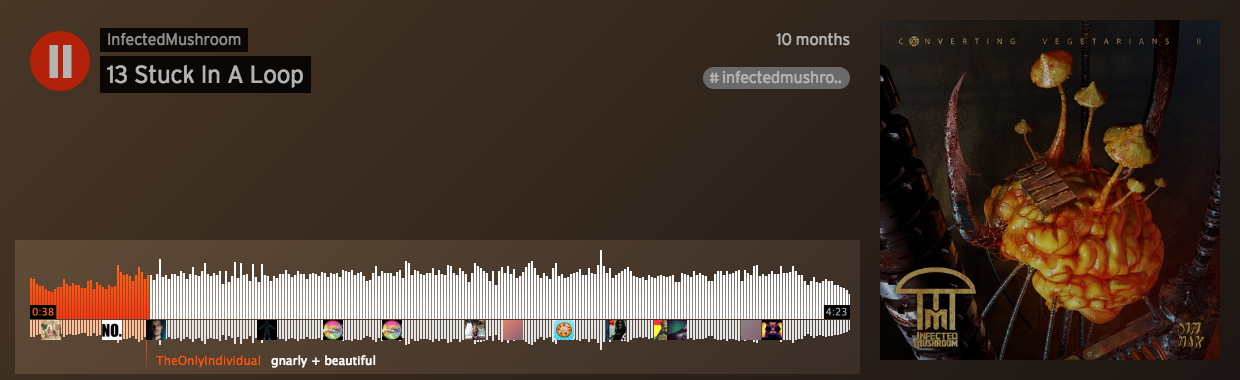
\includegraphics[width=4in]{figures/soundcloud.png}
      \caption{Soundcloud comments. Indicators are embedded into the seek bar}
      \label{fig_youtube_comments}
   \end{figure}

Inspired by these platforms and by the work done in the field of HyperMedia (covered in the Background Chapter), I propose a novel user interface that treats discussion as hyper layers in video. In it, Comments are: 

\begin{itemize}

\item Textual hyper layers on top of the main story video. 

\item \textit{Timestamped} according to the playback time when they're entered and only appear in that time in the playback. 

\item \textit{Discussable}, each one can collapse into it's own thread that allows for further discussion, including text and video messages. 

\item \textit{Indicated} in the video seek bar according to their timestamp.

\end{itemize}

This allows participants to ask questions that relate to a specific point in time and the Organization to answer with rich media, including videos that “drill down”, providing more context in response to a question. It also allows other participants to quickly see where discussions are happening in the video and skim by navigating between them. These properties will be demonstrated in the implementation chapter. <TODO Philipp: more examples of other people working on similar video interfaces>

\subsection{Brainstorming - Collaborative Pads}

As presented in the previous chapter, brainstorming takes many forms. Unlike conversations, which can be modeled as a set of messages, whether directed or broadcasted, Brainstorming also includes the concept of a shared mental model that can be collaboratively manipulated. While this model can live solely inside the head of the participants, it is not a scalable approach. successful models include the use of a medium such as whiteboard, sticky notes, etc. How can we implement such a shared mental model for remote participants?

The usage of a networked computer as a medium that facilitates a shared mental model was first described in 1968 by J.C.R. Licklider. After first attending a meeting in which all participants had a networked computer with access to shared editable resources, Licklider concluded that ``In a few years, men will be able to communicate more effectively through a machine than face to face.''\cite{licklider1968computer}

Nowadays, a common tool to facilitate these shared mental models are real time collaborative text editors. These allow for multiple users to edit the same document at the same time while making changes visible to all other users in near real time. Most of these tools also allow for the tracking of changes, who is responsible for every edit, and provide a discussion mechanism. Some notable editors in this space are include Google Docs\cite{gdocs}, Apache Wave\cite{wave} and Etherpad\cite{etherpad}. 

A real time shared editor fits our needs because it provides a basis for Brainstorming without enforcing too much structure. Given that the range of topics and participants is expected to be wide, the simplicity of text provides an optimal format. 

I propose using collaborative document editing as a basis for Brainstorming. Any participant will be able to propose an idea which then turns into a collaborative text document for collaboratively shaping the idea and discussing it. In the future, these documents could also link to specific frames, comment and comment threads in the video. 
\chapter{Design and Implmentation}
\label{chap_design}

Implementation 

\section{Considerations}:

Given that This is How caters makers and hackers, the technology stack it employs should respect their values of openness and transparency. As such, it must be coherent, extensible and modifiable.
 
This is How will be developed as an open source project. The source code will be available at all stages of development, not just on release, and allow for community contributions. It must utilize open standards, these are governed by transparent standard committees and are royalty free. 

This is How must allow for rapid iterative development. This means using programming languages, libraries and frameworks that value productivity over any other consideration. This also derives extensibility, it must allow for simple integration and composition of third-party open source packages. 

This is How must be familiar. While it is sometimes tempting to use niche programming languages and technologies, these interfere with the ease of community contribution. I prefer technologies with a proven track record and wide adoption rates.

\section{Details}

This is How is developed under the MIT open source license. It is version controlled with the open source GIT /cite{git} version control system and hosted on Github/cite{github} which also tracks bug reports. 

This is How is developed as a web application with three major components: server, client and storage. Both the client and server utilize Javascript as their main programming language. Ther server side uses Node.js, a widely adopted Javascript runtime engine. NPM/cite{}, the most popular Javascript package manager, is used both as a dependency manager and a build system. The server also uses super-glue, described later in this chapter, for video metadata extraction.

ReactJS is The main framework used on the Client side is. React provides a component based, efficient rendering engine and as of writing, is the fastest growing web framework /cite{}. As with the server, NPM manages dependencies although the build process is managed by Webpack /cite{webpack}. For video playback we use the HTML5 <video> tag and for video encoding, the open VP8/cite{} codec. 

Collaborative document editing is done with Etherpad/cite{ehterpad}. Etherpad is a collaborative document editor that was launched in 2008 and released as opensource after being acquired by Google in 2009. It has been in development ever since and is extremely flexible. It can work with a variety of datastores, has built in chat and can be easily embedded into other websites.

Storage is divided into structured and unstructured data. The Structured data includes all conversation and metadata while unstructured data refers to the video files. For structured data we use CouchDB/cite{}, a simple document driven database which allows for real time synchronization between the different clients and the server.  Video files are stored in a simple local file server but can easily plug into 3rd party services such as AWS S3 or Google Cloud Storage.

The Webapp is currently stored on Heroku, A popular platform-as-a-service that makes it dead simple to deploy new versions and scale up and down. However, the usage of open standards and technologies make it simple to migrate to other services or dedicated hardware. 


\section{User Experience Considerations} 

\begin{quotation}
``A user interface is like a joke, If you have to explain it, it's not that good.''
\end{quotation}

The user experience of This is How is based on the three-step process outlined in the previous chapter: discovery, interactive exposition and collaborative Brainstorming. It must be intuitive and rely mostly on common interaction patterns that users are already accustomed to. When introducing novel ideas they must be as self explanatory as possible. 

\subsection{User Experience Overview}

In this section I present the major concepts of the User Experience and overview the experience on a page by page basis. For each of these pages I present the purpose and an overview of the different components. 

\subsection{Main Concepts}

These concepts are used throughout the user experience. Concepts that are local to a specific portion of the experience will be covered in the relevant section.

Users are either participants or organizations seeking help. This is How does not differentiate between the populations thus allowing them to interchange.
Stories are the main entity of the system. Each Story has a main video that describes a process and challenges. Stories also encompass the different collaboration concepts that will be described later.
Tags are terms that represent metadata stories. Each story contains one or more tags. Tags can be manually entered or auto extracted using super glue. 

\subsection{Main Page}

% figure: Main Component. 

The main page serves as an entry page for the system. It allows for browsing stories and filtering by tags. All stories are presented, sorted by the time of their addition on a descending order. These stories are represented as thumbnails with some basic data about the story - title and tags. Clicking on the thumbnail will lead to the story page. In later versions, these stories will be sorted by their level of activity, indicated by volume of recent activity and publication date. 

The main page also allows for filtering. A set of common tags is provided, by clicking on a tag, only the stories with a matching tag will be shown. The first story thumbnail is the add button - Hinting that the user can have their story on this page. Clicking it leads to the Add Story Page

\subsection{Add Story Page}

% figure: Add Story

The Add Story page provides the necessary mechanism for adding a story: uploading a video and providing the necessary details.Video can be uploaded either by clicking on the video area and selecting a file, dropping a video file in it or recording an on-the-fly video, using an attached webcam, by clicking on the \textit{Record} button. Additional data: title, location, description and an initial set of tags, are also required. Clicking the \textit{Publish Now} Button will finalize the process and take the user to their dashboard page. 

\subsection{Dashboard Page}

% figure: Dashboard Page

The Dashboard Page is unique per user and presents a collection of all of their published stories. These are shown as story thumbnails, similar to the ones in the main page. Clicking on any story leads to it's story page. 
Story Page

% figure: Story Page

The Story page is the main tool for facilitating interactive exploration and brainstorming. It consists of two main components: the video component and the idea pad.

\subsection{Video Player}

The video player implements the hyper discussion layar I proposed in the previous chapter. It's basic playback functionality is similar to that of a traditional video player. A seek bar allows for seeking to specific parts in the video and includes a play/pause button and playback time indication.

The video player also includes an always-visible comment input box. When typing a comment, the playback automatically pauses and resumes when the comment is submitted. The submitted comment will be timestamped with the current playback time. Comments appear during playback at their respective timestamp and disappear after a predecided number of seconds. These comments allow participants to contextually ask questions and drill down into the specifics of the story.  

% Figure: Comment threads    

Comments are collapsible into discussion threads. These threads provide a mechanism to other participants and the publisher of the story to explain, clarify and drill down into the story. These threads allow both textual and video replies for the sake of expressiveness. Videos replies can be either pre-recorded or recorded on the spot via a webcam. 

% Figure: Seekbar

All of the comments are indicated as semi-transparents blocks on the seek bar and on mouse hover will display the respective comment. With a glance, it is evident which areas of the video are active in terms of discussion and provides a seeking mechanism for the author and other participants.  
\subsection{Idea Pad}

% Figure: Idea Pad

The idea pad accommodates brainstorming by allowing participants to suggest ideas. Initially, an idea is entered as an idea title. Rather than discussing these ideas as simple conversations, they collapse into collaborative documents which any user can share and help evolve. These documents also contains a discussion pane in order not to pollute the document with traditional conversation. 

These ideas can be voted up and down by other participants, a common practice in Q\&A services/cite{stackoverflow}/cite{quora} that allows for the community to bubble up the worthy ideas.   

\section{SuperGlue - MetaData extraction}
SuperGlue is an automatic metadata extractor that works with all forms of media: video text and sound. It is a core project and an ongoing research effort at the Viral Communications group. It serves as basis for exploration of media and enables the next generation of media-centered application.

SuperGlue is built as a modular, expandable system that forms an analysis pipeline. Media is submitted on one side of the pipe and at its end, a rich metadata document is generated and stored on a shared databases. The modules themselves range from face detection to transcription and natural language processing. Modules can declare dependencies on other modules. For example, the natural language keyword extraction module depends on the output of transcription module.

While originally being designed for processing of news, as demonstrated in This is How, SuperGlue can handle various types of Media. For This is How, we utilize the keywords extracted from from transcript. From empirical testing, we've concluded these tend to have a high relevance score.    

\subsection{SuperGlue Implementation}

Superglue has 4 main components: an api server, a task queue, workers, and a datastore. 

The API server is a simple webapp written in Python. It's job is to mediate between the application that use SuperGlue as well as receive submissions of new media items and placing them in the task queue. The task queue is implemented as a Redis database with one value: a simple ordered list of tasks. Each task represents one module that needs to run on one media item. These tasks are inserted either by the API server or the workers. 

The Workers are the main work horse behind the system and are also implemented in Python. Modules are defined with python classes that adhere to a simple module api. As part of the definition, they can also declare dependencies on other modules. Whenever a worker is free, it polls the task queue for the next task. It then executes the relevant module on the relevant media item and stores the result in the database. Upon completion, it will detect which modules depend on the one that just completed, and will insert new tasks for all of them in the task queue. 

% Figure: A fancy graph showing modules

All the data is stored in a single collection in a MongoDB database. Each record in this collection represents a single media item and all the output that's been gathered from the various modules is stored in it. 

This architecture results in an ability to successfully scale horizontally. Workers, which are the main units of computation, are stateless and as such can be added and removed without affecting the system. SuperGlue is currently processing 500 hours worth of video in a day using 20 workers running on virtual machines.
\chapter{Evaluation}
\label{chap_eval}

In chapter X, Anatomy of bla bla, I concluded that the process of story­centric brainstorming and collaboration works towards the goals mentioned in the introduction section. Nonprofits have had valuable insights by working with makers, they have learned about their unique skillsets and collaborated towards solutions. Makers, in turn, practiced their skillsets and gained confidence in their abilities.

In this chapter, I focus on evaluating the move from ``real life'' collaborations to online collaborations using the newly built T  his is How platform. I start by evaluating the video medium itself and then examine the platform itself by means of comparison to the test cases presented in Chapter 3.

Video ­ Sanity Check

Before building  This is How, as a preliminary study, I tested the effectiveness of video as a medium with a group of makers. I produced several short videos telling the story of the nonprofit Cradles to Crayons, mentioned in chapter 3. This story was comprised of a two minute overview video describing the nonprofit and three short videos describing specific challenges. A static website was built, containing these videos. The webpage, along with the videos were shown to a group of makers in the South End Technology Center (SETC) in Boston.

% Figure of web page

The SETC is a makerspace, a part of the global fablab /cite{fablab} network of maker­spaces. SETC is unique in that it is operated by high school students. The students take part in a program called ``Learn to Teach, Teach to Learn'' in which they both learn fabrication skills and pass them on to the community and other students throughout the year. During the summer, the students work on projects that utilize the different skills they've learned.

I joined one of the weekly classes these students attended and presented the Cradles to Crayons story through the webpage mentioned above. The main video was shown, along with one of the challenges video. I myself did not add any information beyond the videos shown. I then opened a discussion by asking the students what they learned about the nonprofit and how they could utilize their skills to help it. Although some of the students already knew about the nonprofit, they were still surprised to learn about the complexities of running its operations. They then expressed interest in working on projects that might help in dealing with the challenges faced by the nonprofit. These project proposals beared a surprising resemblance to the ones proposed by other makers in the onsite visit described in Chapter 3.

   \begin{figure}[thpb]
      \centering
      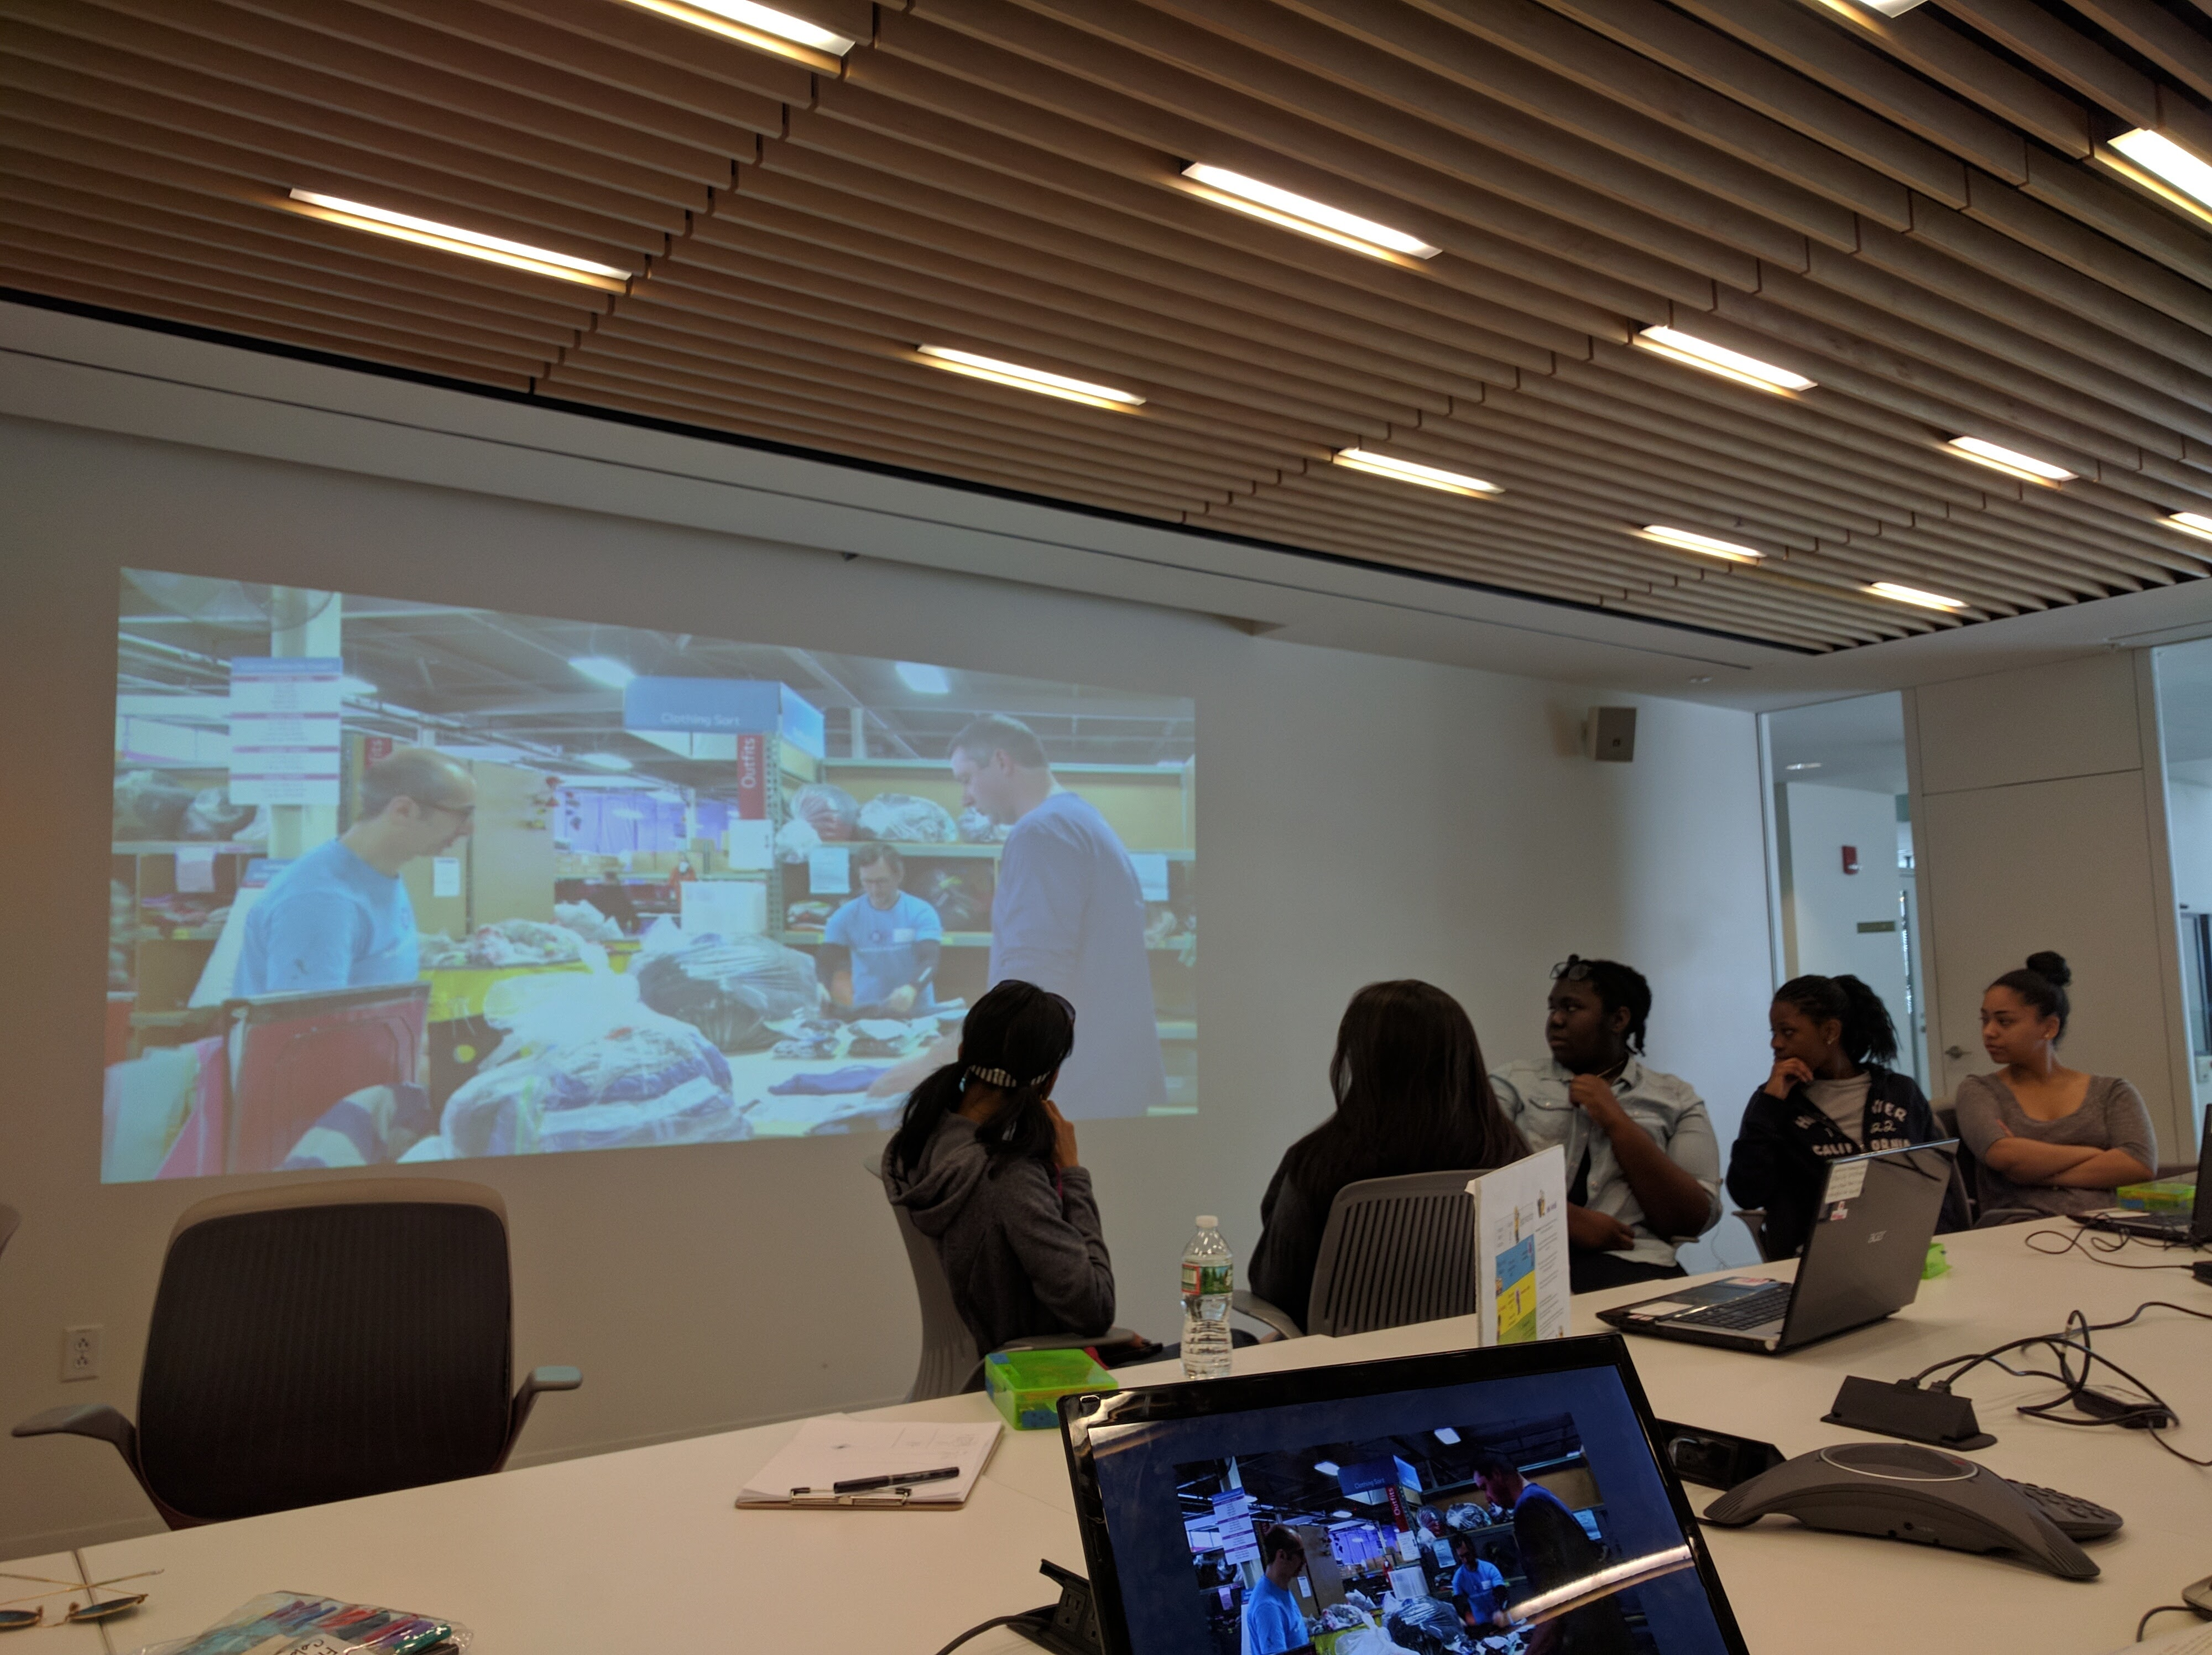
\includegraphics[width=4in]{figures/learn2teach.jpg}
      \caption{Presenting the Cradles to Crayoto story at a \textit{Learn to Teach, Teach to Learn} session}
      \label{fig_setc}
   \end{figure}

Later that day, Susan Klimczak, who runs the program, sent me an email regarding the visit which included the following:

\begin{quotation}

``When we did feedback, 5 of the youth talked about how meaningful it was to have you come in \& do the cradles to crayons! They said that it would be very valuable to have you come in regularly to present real community issues that need to be solved.''

\end{quotation}

Even without the components of interactivity and collaboration towards a solution, it was clear that the video achieved two important goals. First, it managed to raise awareness for the nonprofit, and second, it empowered the makers by providing a real world example of the value of their skills.
User Studies ­ This is How

I've conducted structured interviews (Appendix) with all three nonprofits mentioned in Chapter 3 as well as three makers who participated in some sort of collaboration with them. These nonprofits vary in scale and in type of operation.

\section{User Experience Evaluation}

The user experience evaluation centered around a demonstration given by my self. The demonstration started from the main story page, including commenting and idea pads, and then moved on to browsing and story creation. 


Per step, the interviewee was requested to rank the ease of use, according to their personal experience. They were also given an option to elaborate. I present a summary of each of the steps.

\subsection{Video}

\subsection{Story Comments System}

The subjects were shown an existing video story with comments, and comment replies, both in the form of text and video.

There was a unanimous agreement between subjects that once an existing comment in the video appears, the timeline-based discussion is self explanatory. Some of the interviewees stated that clicking on a comment to open the reply-to-comment system is not intuitive, However, once having seen it, the options to reply by text or video are self explanatory and valuable.

Makers and nonprofits alike have stated that this step seems to be true to the purpose of interactive exploration, as experienced in their collaborations. Some subjects thought the asyncronous nature of the online discussion has more potential than real life interactions because it gives the parties a chance to think about their replies. Others stated the opposite, that the asyncronous nature removes a sense of urgency which exists in real-life discussion and drives it. 

\subsection{Story Creation}

This step focused on the nonprofits, being the story creators, which all stated that the form and mechanics of uploading a file were straightforward and self explanatory, including the usage of tags as keywords. 

This step also served as a trigger for discussion regarding the feasibility of producing a compelling video story. The two smaller nonprofits stated that they believe it's within their reach to produce such a video while C2C, the largest and most established one, raised a concern regarding video quality. All media released to the public domain by them must be vetted to comply with the organization's public relation's team which has high standards.   

\subsection{Idea Pad}

The subjects were shown an Idea Pad with existing ideas regarding the same story as the previous section. Some of these ideas have already been collaborated on and discussed on by various users.

All the nonprofits stated that it is hard to evaluate without real usage although it seems to be straightforward and fits the process of brainstorming. C2C, the larger nonprofit and also the most aware of public relations, was worried that non-makers who visit the page, will not understand the goal of the idea pad.   

Two of the makers appreciated the lack of structure in the pad as a tool for free form brainstorming while the third was worried of the exact opposite, that the lack of structure does not accommodate the relationships between ideas.

\subsection{Browsing}

The subjects were shown the main page along with the option to filter by tags.

Nonprofits were neutral in their response while makers expressed a concern about scalability, how the page well look like with many stories, including the lack of a free form search option.

\subsection{Overall User Experience}

Makers and nonprofits alike have stated that in general the user interface provides a concise and self explanatory experience. The novel components, including the commenting system and the idea pad, become clear once they saw them populated with data.     


\section{"This is How" as a platform}
Subjects were asked whether they believe 
\chapter{Conclusion}
\label{chap_conclusion}

The goal of this thesis was to foster collaboration between the maker community and nonprofit organizations. This was done through two main contributions. 

First, an outline of the process of story­ centric brainstorming and collaboration was presented. Through examination of case studies and interviewing the parties involved I demonstrated that these type of collaborations contribute to the stated goals. Makers gained confidence in their skills and their ability to make an impact, and nonprofits gained different perspectives on the challenges they face, collaborated towards solutions and learned about the maker movement. 

Second, I designed and implemented a web application, \textit{This is How}, that distributes the outlined process by using HyperMedia as a method for interactive exploration and collaborative idea documents as basis for collaboration. By interviewing the same nonprofits and makers from previous examples regarding \textit{This is How} I established that it has the potential to replicate the process of story­ centric brainstorming and collaboration in a distributed manner.     

\section{Limitations}

\subsection{Storytelling through video is not easy}

The stories in \textit{This is How} are based on videos which need to strike a balance between telling a compelling story, having enough details to attract makers and yet refrain from being cumbersome. While the three nonprofits covered in this thesis have stated that they believe creating such a video is within their capacity, that is yet to proven. I think the guidelines presented in the previous chapter are a good starting point and I'm encouraged by how well these nonprofits are in presenting their story in person. I believe that with an initial corpus of successful videos in the system, nonprofits will be able to utilize imitation as a tool for creating a compelling video story.

\subsection{Variance in the Maker movement}

Most makers interviewed in this thesis are from the MIT network, they are extremely capable and socially aware. However, The very definition of a Maker is undefined, Makers range from expert engineers in various fields to kids in elementary school practicing arts and crafts. More than that, the motivation for engaging in ``making'' is also varied, from personal expression to social activism and more. 

Having visited various maker spaces in the greater Boston area I believe that the best candidates for \textit{This is How} are makers that are already organized in frameworks with a tendency for social good, such as the previously mentioned \textit{Learn to Teach, Teach to Learn} program. To jump start \textit{This is How} it is crucial to connect and collaborate with these organizations.

\subsection{Variance in Nonprofits}

The three nonprofits covered in this thesis differ greatly from one another but still represent an extremely small sample size. Nonprofits vary in size, characteristics of operation and numerous other factors. Many of them focus solely on the distribution of money and have no use for the maker skill set and some bigger nonprofits, such as \textit{Cradles to Crayons}, work at a scale in which it is harder to experiment and have other considerations such as public relations.
It is clear that for a nonprofit to benefit from a platform such as \textit{This is How} they should be small enough to allow experimentation and have a ground operation that benefits from the maker skill set. As the system grows, the characterization of an ideal nonprofit candidate will be refined.   

\subsection{Single Iteration} 

This is How in it's current form is a first iteration. In the world of software development, especially software that's provided as a service like web applications, it is necessary to observe users' behavior and constantly refine and validate both the underlying assumptions and the specifics of user experience.

\section{Future work}

The next main step for This is How is deployment. Evaluating the system with a small set of nonprofits and makers has been invaluable for the development process but can not be considered a predictor for success.

Deployment requires more than just opening the system up for the general public, it requires building and maintaining a community. This entails actively seeking relevant nonprofits and helping them tell their story in a concise way that can allure makers. 

Deployment also means to approach maker communities, both virtual and physical, and promote the system. Hopefully, with a critical mass of stories and ongoing collaborations, the existing users, both makers and nonprofits, will be the ambassadors of the system and attract their peers.

\section{Reflections}

Working on this thesis has had a tremendous impact on me.

Collaborating with nonprofits has taught me many lessons about humility and selflessness. My trips to various nonprofits and the meetings with their employees and volunteers kept reminding me of the importance of my work but more than that, they served as a much needed moral compass for a student spending most of his time in the meritocracy of MIT.

I was also inspired by my visits to maker spaces, outside of MIT, where the sparse resources led to creative thinking. I was reminded what it means to learn and to build out of curiosity rather than out of a requirement to innovate. Getting a positive response from the kids of the South End Technology Center was probably the most exciting moment in this entire process.

With that said, there were also many days and weeks spent on directions that turned out to be dead ends. At times, I was frustrated by lack of success in enlisting makers and nonprofits, to the point of questioning the basic assumptions of this thesis.

Moving forward, I still can't say if I'm going to proceed with this project but I know for sure that it will stay with me wherever I go.
% 
% introduction
%  - vision/overview
%     - a decade from now robots will take the place along side humans and animals
%     - as companions, playmates, tutors, assistants
%     - there is a change in what we have to be, what we have to regard as peers to make this happen
%     - john henry vs robots
%  - why empathy for robots
%  - theory of life story
%  - description for rest of thesis


\chapter{Introduction (TEX Reference/Palash)}
\label{chap_intro_ref}


   \begin{figure}[thpb]
      \centering
      \includegraphics[width=4.6in]{figures/intro/tears_in_the_rain.png}
      \caption{Death of a replicant in the movie \textit{Blade Runner}}
      \label{fig_ec_story_no_story_lm}
   \end{figure}


What makes us human? This question is explored in the science fiction movie \textit{Blade Runner}. Set in a future-noir world against a backdrop of neon lit skyscrapers, we take on the persepctive of Deckard who is tasked with hunting down and killing replicants, an organic artificial humanoid. The replicants are assumed to be not human, a premise supported by their lack of moral rights. The movie suggests that what makes us human lies in the difference between the two. 

However, from this beginning, the movie systematically eliminates possible candidate differences: physical form, intelligence, motivation to survive, emotional experiences, and so on. The last ontological distinction is lost at the death of the lead replicant. In one of cinema's most memorable scenes, just before his death, the replicant says:

\begin{quotation}

``I've seen things you people wouldn't believe. Attack ships on fire off the shoulder of Orion. I watched C-beams glitter in the dark near the Tannh\"{a}user Gate. All those moments will be lost in time, like tears...in...rain. Time to die.''

\end{quotation}

As he dies, in an allegorical reference to the ascension of a soul, a dove leaves his hands and flies up into the light. What was lost at death was, in his own words, his unique experiences that we could only glimpse but not fully know. At that moment, we cannot help but feel moved by the death of the replicant \cite{rowlands_philosopher_end_universe}. The movie merges the ontological categories by having Deckard, who we had identified with, realizing after this scene that he might be a replicant himself \cite{mulhall_blade_runner}. 


Relating to and being emotionally engaged by life-stories of machines is a recurring theme in many science fiction works: \textit{2001: A Space Odyssey}, \textit{Ex Machina} and \textit{Otherspace}, to name a few. This thesis is an exploration of this theme.



\section{Research Question}

The main research question of this thesis is whether the implicit life-stories of a robot can invoke empathy for it. By implicit life-stories I mean the ability of the robot to experience the world we live in, to be transformed through that experience, and  to communicate the experience to us. By empathy for a robot, I mean understanding and experiencing the robot's perceived emotions as if they are our own. 

%
% Science fiction encourages us to imagine a world where we have companion robots that live alongside us and participate in our daily lives. Suspension of disblief is requested by placing this world in a distant future or in a galaxy far far away. However, this future isn't as foreign as these literary devices suggest. It is my belief that we are within a decade of having robots in our homes that can be companions, playmates, tutors and assistants. These robots may serve us, entertain us or teach us but most importantly we would find a sense of social other in them. One important aspect of relationships we have in our lives with either other humans or companion animals is that we feel empathy towards them. In this work, I propose one design critera for creating companion robots: giving robots an implicity life-story: the ability to experience the world, change through that experience and communicate it to us in a relatable way. I show that this ability encourages us to have empathy for the robot. 


\section{Why Empathy for Robots?}


   \begin{figure}[thpb]
      \centering
      \includegraphics[width=4in]{figures/intro/gray_dimensions_mind.png}
      \caption{Gray et al.'s analysis of people's perception of minds of various character showed that robots are considered to be lacking in experience compared to other characters \cite{gray_dimensions_mind}}
      \label{fig_intro_gray}
   \end{figure}
   

Empathy for artificial agents has been proposed as a test of believability; that is to say, the greater the ability an agent has to invoke empathy, the more it is perceived  to be life-like \cite{paiva_empathic_virtual_agents}. A common conception of robots is that they do not have the capacity for emotions. Gray et al. examined people's perception of minds by asking participants to rank characters on various mental capacities (for example, out of a robot and a baby, which has greater capacity for pride, for telling right from wrong, etc.) and personal judgements (for example, who should be more deserving of blame if they were to cause harm to others) \cite{gray_dimensions_mind}.  Analysis of the responses showed that while robots were perceived to have agency that is comparable to other living entities, they were most lacking in affective experiences (See Figure \ref{fig_intro_gray}).  If we have empathy for robots, that is to say, we feel that we experience their emotions as if our own, then I argue that we implicitly believe that such robots have emotional experiences. Such capability could elevate the perception of robots to be closer to that of other living creatures. The process of bringing robots closer to us in our perception is, by construction, a pursuit of trying to understand who we are. 



   \begin{figure}[thpb]
      \centering
      \includegraphics[width=4.6in]{figures/intro/paro_large.jpg}
      \caption{Residents at a retirement home find comfort in Paro, a therapeutic robotic seal\cite{nbcnews_paro}}
      \label{fig_intro_paro}
   \end{figure}
   

    A second case for empathy towards robots is to create robots that can have roles similar to companion animals. There is wide evidence that companion animals have a beneficial effect on our physiological and psychological health. Interaction with companion animals has been shown to reduce loneliness, blood pressure, cholestorol, depression, anxiety, and stress \cite{walsh_human_animal_bond}. An important aspect of our relationship with animals is that we tend to feel empathy toward them. \cite{phillips_empathy_animals}. In addition, empathy toward companion animals can lead to greater empathy toward humans, which is a highly prosocial trait \cite{gullone_empathy_prosocial_pets}. It is worth exploring how to design robots to elicit empathy which could bring some of the benefits of companion animals to those who are unable to have them.


%Empathy for artificial agents has been proposed as a test for believability ie. life-likeness \cite{paiva_empathic_veritual_agents}A common perception of robots is that they cannot have experiences of pain, pleasure or joy. This perception is related to personal judgements that robots are not deserving of moral rights or do not have a soul \cite{gray_dimensions_mind}. If we have empathy for robots, that is to say experience their emotions as if our then I argue that we implicity believe that such robots have emotional experiences. Such capability could elevate the perception of robots to be closer to that of other living creatures. This process of bringing the robot closer to us in perception is really a pursuit of trying to understand who we are by construction.


% robot as a tool for understanding who we are
% empathy for robots will inform robot's moral rights


\section{Implicit Life Stories}
\label{sec_intro_theory}

Living entities grow and change from experience over the course of their lives. Dautenhahn and Nehaniv described life as a complex story embedded in biology \cite{dautenhahn_nehaniv_alife}. Changes in morphology or behavior tell the story of the object. For example, consider encountering an one-eyed orange cat sunning itself on a wall. From that brief encounter, one extrapolates a checkered past of scuffles in alleyways and summers enjoying warmth. While I leave more to the reader's imagination, the point here is that through morphology and behavior, living creatures implicitly tell the stories of their lives. 

However, these stories are told imperfectly. They are not simple reproductions but rather underspecified ambiguous descriptions. Underspecificity, Gaver argued is a virtue, as it engages us as particpants \cite{gaver_ambiguity}. We become particpants in constructing the story. Ackermann wrote that viewers engage with objects by ``reconstructing them through the lens of their own interests and experiences.'' \cite{ackermann_experience_artifact} We color in the details of the stories using our own life-stories. We wince at the pain of the imagined fight that cost our orange cat his eye from past experience of our own pain. Empathy is generally defined as the ability to understand and feel what another feels \cite{decety_human_empathy}. If, through our own experience, we understand and are engaged by the experiences of another, then it stands to reason we would feel empathy for them. I posit that if we can build robots with implicit life-stories, we will feel empathy towards them. 

Based on the argument I outlined, I consider the following properties necessary for a robot to have an implicit life-story:

% By implicit-life stories I mean the ability of the robot to experience the world we live in, to be transformed through that experience, and  to communicate the experience to us. Empathy here means understanding and experiencing the robot's emotions as if they are our own.
\begin{itemize}
\item Autonomous agent: Robot can mean different things. For the purpose of implicit life-stories, all that is required is the robot is perceived to be capable of sensing and acting on the world driven by an internal process. This is necessary to be able to attribute experience to it. 
\item Perceptible change: The robot must change from experience. Without change, experience wouldn't leave an imprint on the robot. The change needs to be human perceptible so we would know of its existence and of the experience that caused it.
\item Relatable experience: The change to the robot must come from an experience that we could imagine ourselves having. A machine learning algorithm, learning to classify a dataset, is changing from experience but an experience we cannot share. Such an agent wouldn't qualify as having an implicit life-story by my definition. Embodiment and/or having human-like perception would make it easier for an agent to have a shareable experience.
\item Ambiguous Experience: As discussed earlier, the change to the robot must ambiguously reflect, or evoke, the experience it had. A video camera recording a movie is changing from a perceptual input that we could have. However, the perfect reproduction doesn't leave room for us to imagine a social model much less being able to put ourselves in its place. On the other hand given an input, the resulting change cannot be incomprehensible as that would preclude us from reconstructing the experience. 
\end{itemize}


Over the next few chapters, I share what I learned from building robots according to these ideas and testing my thesis with human subject studies. 


\section{Thesis Overview}

\hspace{7pt} Chapter \ref{chap_background}: I provide background for social robotics and empathy and describe the relationship of this work to these fields. I also note related work done on stories for artificial agents.

Chapter \ref{chap_lightbug}: I describe a minimal robot that I construct as a preliminary exploration
of implicit life-stories. Consider this as a thought experiment. 

Chapter \ref{chap_hexbug}: I test my thesis with a human robot interaction study where participants interact with a toy robot that has been given a fictional implicit life-story. After the interaction, the participants are asked to strike the robot. From measuring their hesitation to strike and through psychometric tests, I show that life-stories invoke empathy.

Chapter \ref{chap_design}: Based on the results from the initial human subject study, I build a sound robot that can have a life-story. In this chapter, I describe design considerations, the process of building the mechanical systems, and the architecture of the software necessary to animate the robot and to learn sounds. 

Chapter \ref{chap_pilot}: I then conduct pilot studies with human subjects to understand perception of the robot and to refine validation study design. I describe my experience of iterating on the design. 


Chapter \ref{chap_study}: I conduct controlled human subject study with both online and in person participants. I show that implicity life-stories create greater empathy for the new robot. I also find that empathy for robot can impact subsequent empathy for humans. 

Chapter \ref{chap_final}: I summarize my findings from my studies and my contributions to the field. I discuss ideas for extending this work and possible applications for such robot.



\section{Contribution}
As a preview of the final chapter, I submit these as my contributions:


\begin{itemize}
\item Proposed a new design element, implicit life-stories, for engendering empathy for social robots
\item Demonstrated empathy for robots with implicit life-stories through human robot interaction experiments across two different platforms
\item Designed and built a novel sound interaction social robot to embody and test these ideas
\item Demonstrated that the implicit life-stories can improve perception of social robot on animacy, anthropomorphism, likeability and intelligence measures
\item Showed that empathy for robot has an impact on subsequent empathy for humans. This is the first work to examine the connection between the two.
\item Open-sourced design and code for the new robot
\end{itemize}






%%%%%

%\section{In Popular Culture}
% - talk about recurring occurence of memories as the key part of movies about robots
% - talk about hitchbot and stories

% I am certainly not the first to suggest that a machine that can have experiences is emotionally meaningful to us. There are numerous references to such
% a notion in popular culture. In the movie, 2001 a space odyssey, there is a powerful scene where Dave is dismantaling Hal's memory bank. As
% Hal looses his memory he regresses and starts to recite nursery rhymes. Watching the scene there is a sense of a loss of a sentient being and one cannot
% help but feel sad for Hal. 

% In another movie, Blade Runner, just before death during poignant scene, the main antagonist, Roy Batty, laments that all his unique experiences will be lost.
% In an allegorical moment a dove escapes from his hands and flies off into the sky. This is regarded as Cinema's top 100 memorable scenes. The allegory refers
% to the flight of his soul. The corporal body remains and in the case of robots, believed to perfectly resuable, but the memories are gone.  These
% reflect this sense that it is the memory and the experience that matters. One sees motif repeated in science fiction but also in real life. 

% When the canadian hitch-hiking robot, HitchBot, got violently dismembered and tossed into a garbage dump, there was an outpouring of sympathy. 


% One of science fiction film's most dramatic moments is the death scene of an android, Roy Batty, in the movie Blade Runner. The movie is set in a
% world inhabited by humans and also androids. The androids while appearing human and having intelligence and even capacity for emotions are regarded
% as distinct from humans and impassionately hunted down and killed. However, in a climatic scene, the lead android is about to pass away and before
% pasisng he recounts his experiences in a famous soliliquoy: ``I have seen things you people wouldn't believe... c-beams glitter in the darkness...
% all these will be lost in time...'' It's a transforming moment. At that final brief moment, Roy seems human and one feels sad for him. THe crew 
% reportedly wept at the scene. 

% What I find fascinating here is that final humanizing moment, what the character puts forward is his story. This is the final bit that makes him relatable
% and invokes empathy for him. 


% Have you seen the movie Blade Runner? The science fiction movie is set in a world populated by humans and androids that look exactly human and behave almost similarily to the point that it is difficult to tell them apart from humans. A cenral theme of rhte movie is trying to understand how teh androids are not human or that is to say that what makes us different from robots. Do androids have a soul or are they just amchines? Near the end of the movie, there is a climatic scene, one of the most memorable ones in cinema, where the lead android, the antagonist dies. As he dies he says " I have seen all these things, you people wouldn't believe...." And at his death, a pigeon flies into the sky in allegorical scene as if his soul is leaving the body. What I find poignant is what is lost are the memories and experiences of this android described ambiguously in this beautiful solilquoy. The soul of the machine are these experiences. 

% This is a theme that is repeated in many science fiction descriptions of fictional AI: 2001 a space odyssey, ex machina, other space. Perhaps the anime that we seek to imbibe robots with is in the ability of the robots to create life-stories. 



\newpage\null\newpage


% ********************************************************************
% Backmatter
%*******************************************************
\appendix
\renewcommand{\thechapter}{\alph{chapter}}
\cleardoublepage

% CHANGE THIS - palash
% (add appendices if any)
\chapter{Appendix - SuperGlue API}
\label{appendix}

\section{Posting media to SuperGlue}

\section{Querying metadata from SuperGlue}


%********************************************************************
% Other Stuff in the Back
%*******************************************************
\cleardoublepage\include{FrontBackmatter/Bibliography}

% ********************************************************************
% Game Over: Restore, Restart, or Quit?
%*******************************************************
\end{document}
% ********************************************************************
